\documentclass[11pt]{book}
\usepackage[utf8]{inputenc}
\usepackage{longtable}
\usepackage{color}
\usepackage{multirow}
\usepackage{hyperref}
\usepackage{setspace}
%\doublespacing

\renewcommand*{\sectionautorefname}{Section} 

\title{E1} 
\author{Raphael Klein}

\usepackage{natbib}
\usepackage{graphicx}
\usepackage[labelfont=bf]{caption} 	% Make captions bold (Figure & Table)
\usepackage{subfig}	
\usepackage{amsmath}
\usepackage{hyperref}
%\usepackage[section]{placeins}

\providecommand{\keywords}[1]{\textbf{Keywords:} #1}

\begin{document}

\maketitle

%\textcolor{red.green.blue.cyan.yellow.magenta.}{}

%\newpage

% structure of the report
% Introduction
% Modelling
%	Electricity model
%	Policy emergence model (SM)
%	Hybrid model
% Implementation
%	Electricity model
%	Policy emergence model (SM)
%	Hybrid model
% Code documentation
%	Electricity model
% 	Policy emergence model (SM)
%	Hybrid model
% Verification
%	Electricity model
% 	Policy emergence model (SM)
%	Hybrid model
% Inputs
%	Electricity model
%	Policy emergence model (SM)
%	Hybrid model
% Experimentation - Scenario design
% Model initialisation
%	Electricity model
% 	Policy emergence model (SM)
%	Hybrid model
% Model results 
% Conclusions

\tableofcontents

%%%%%%%%%%%%%%%%%%%%%%%
\chapter{Introduction}
\input{Introduction}

%%%%%%%%%%%%%%%%%%%%%%%
\chapter{Modelling}
\section{The electricity model}
\label{sec:CodeDocElec}

The model presented in this chapter is a transposition of the model created by Paul van Baal and Reinier Verhoog and first created by Paul van Baal for his master thesis \citep{van2016business}. The model has also been further improved to look into the effect of a strategic reserve in a hybrid system dynamics - agent based model version \citep{van2019effectiveness}. In this report, the model, which was a system dynamics model and then a hybrid model, is turned into an agent based model. This report is the ODD presentation of that model \citep{grimm2010odd}. All equations and additional details are in the appendices.

%%%%%%%%%%%%
\subsection{Purpose of the model}
\label{ssec:purpose}

The purpose of this model is to simulate the Swiss electricity system. This includes the spot market, international trade with neighbouring countries, and investments. This constitutes what is considered to be the simplest electricity model (SMel). In future iterations of the model, depending on the goals of the research, the model can be extended to consider the presence of demand side management, batteries, prosumers or a strategic reserve.

%%%%%%%%%%%% end of subsection

%%%%%%%%%%%%
\subsection{Entities, state variables and scales}
\label{ssec:entities}

There are four types of agents within the model: the market operator, the firms (or investors), the supply agents and the demand agents. The market operator is the agent that is in charge of the spot market, making sure everything is going well. The firms are the agents that own the power plants and other assets present in the model. They are in control of the  power plants. The demand agents are the agents that buy electricity. This includes the inflexible demand (which is based on a  historical scenario), and demand created by hydro-pumping power and international trading.

%There are two types of agents within the model: the agents which are in charge of taking care of the electricity market and the assets which represent the physical infrastructure and which produce electricity.

The firms are characterised by the following attributes: assets owned, electricity supplied, planned assets, retired assets and constructed assets. The supply agents can either be the power plants (assets), they can be long term contracts with France, or they can be the net transfer capacities from the different border countries. Each has a different set of attributes. The assets are characterised by the following attributes: owner, technology type, installed capacity, age, lifespan, capital costs, annual fixed costs, variable costs and utilisation factor. Additionally, depending on the technology type, some power plants have more parameters. For example, the thermal power plants, the nuclear power plants and the waste power plants all have a fuel cost. The thermal power plants also have an emission attribute. The nuclear power plants have attributes related to their maintenance requirements: maintenance month and maintenance time. Waste, hydro and hydro-pumping assets have attributes related to their reservoirs: reservoir level and maximum reservoir level. Hydro-pumping assets have an efficiency attribute related to their pumping efficiency.

The technology types are limited to: solar, wind, hydro power, hydro-pumping power, run of river, thermal, nuclear and waste. The firms can only invest in solar, wind and thermal technologies as it is considered that other technologies are already maxed out in Switzerland or they cannot be used to produce significantly more electricity.

%The actors are provided as follows: the market operator, the firms, the supply agents and the demand agents. The market operator is the agent that runs the spot market. The firms represent the investors that have the capacity to invest for new generation capacity. They also have to decide whether to keep plants online, if they should be mothballed or dismantled. The supply agents are the plants themselves but they can also include foreign countries. Finally, the demand agents create the electricity demand that represents the demand in Switzerland but also the demand of hydropower pumping plants.

%%%%%%%%%%%% end of subsection

%%%%%%%%%%%%
\subsection{Process overview and scheduling}
\label{ssec:process}

The model runs along two different scales, highlighting two parts of the model. The first part is the spot market, running on an hourly basis. It consists of all the actions related to the spot market including all of the inputs, the calculation of the demand, the calculation of the spot price, the distribution of the money and electricity when the equilibrium is found and the update of the NPV for all of the agents (that is later used for investments).

The second part is related to the investments that the firms can perform. This happens monthly. These are actions that are related to the firms. They decide whether to invest in new assets. They also decide whether they should reinvest in their current assets by extending their lifetimes or shuttering them temporarily or definitively. Then there are additional measures that include the end of life actions that occurs when an asset has reached its lifetime. It also includes scenario based events such as the closing of nuclear power plants according to a politically determined timeline.

%%%%%%%%%%%% end of subsection

%%%%%%%%%%%%
\subsection{Design concepts}
\label{ssec:design}

%%
\paragraph{Basic principles}
%Which general concepts, theories, hypotheses, or modeling approaches are underlying the model?s design? Explain the relationship between these basic principles, the complexity expanded in this model, and the purpose of the study. How were they taken into account? Are they used at the level of submodels (e.g., decisions on land use, or foraging theory), or is their scope the system level (e.g., intermediate disturbance hypotheses)? Will the model provide insights about the basic principles themselves, i.e., their scope, their usefulness in real-world scenarios, validation, or modification (Grimm, 1999)? Does the model use new, or previously developed, theory for agent traits from which system dynamics emerge (e.g., ?individual-based theory? as described by Grimm and Railsback [2005; Grimm et al., 2005])?

The model is, in essence, a simple supply and demand model where electricity is demanded and supplied. The main added element is that instead of resolving this supply and demand every week or year as it has been done in past models, it is done on an hourly basis.

%%
\paragraph{Emergence}
%What key results or outputs of the model are modelled as emerging from the adaptive traits, or behaviours, of individuals? In other words, what model results are expected to vary in complex and perhaps unpredictable ways when particular characteristics of individuals or their environment change? Are there other results that are more tightly imposed by model rules and hence less dependent on what individuals do, and hence ?built in? rather than emergent results?

The main outputs of the model relate to the energy mix that is needed to meet the Swiss electricity demand. The investments, their type and amount are also of interest for the purpose of the study and should emerge from the needs to supply electricity.

%%
\paragraph{Adaptation}
%What adaptive traits do the individuals have? What rules do they have for making decisions or changing behaviour in response to changes in themselves or their environment? Do these traits explicitly seek to increase some measure of individual success regarding its objectives (e.g., ?move to the cell providing fastest growth rate?, where growth is assumed to be an indicator of success; see the next concept)? Or do they instead simply cause individuals to reproduce observed behaviors (e.g., ?go uphill 70\% of the time?) that are implicitly assumed to indirectly convey success or fitness?

There is no real adaptation programmed in this model beyond agents deciding on whether to discontinue their current assets and whether to invest in current or new ones.

%%
\paragraph{Objectives}
%If adaptive traits explicitly act to increase some measure of the individual?s success at meeting some objective, what exactly is that objective and how is it measured? When individuals make decisions by ranking alternatives, what criteria do they use? Some synonyms for ?objectives? are ?fitness? for organisms assumed to have adaptive traits evolved to provide reproductive success, ?utility? for economic reward in social models or simply ?success criteria? (note that the objective of such agents as members of a team, social insects, organs ? e.g., leaves ? of an organism, or cells in a tissue, may not refer to themselves but to the team, colony or organism of which they are a part).

The objectives for the market operator is that there be a balanced spot market. The objective for the firms is to make as much money as possible. The objective of the supply agents is to supply as much energy as possible. The objective of the demand agents is to have their demand met. 

%%
\paragraph{Prediction}
%Prediction is fundamental to successful decision-making; if an agent?s adaptive traits or learning procedures are based on estimating future consequences of decisions, how do agents predict the future conditions (either environmental or internal) they will experience? If appropriate, what internal models are agents assumed to use to estimate future conditions or consequences of their decisions? What tacit or hidden predictions are implied in these internal model assumptions?

The firm agents have to use prediction for the investments. They forecast the price of electricity for the next year, two years and five years based on historical data for each technology considered. This is then used in the profitability check and the Net Present Value (NPV) by the firms for their respective assets or future investments.

%%
\paragraph{Sensing}
%What internal and environmental state variables are individuals assumed to sense and consider in their decisions? What state variables of which other individuals and entities can an individual perceive; for example, signals that another individual may intentionally or unintentionally send? Sensing is often assumed to be local, but can happen through networks or can even be assumed to be global (e.g., a forager on one site sensing the resource lev- els of all other sites it could move to). If agents sense each other through social networks, is the structure of the network imposed or emergent? Are the mechanisms by which agents obtain information modelled explicitly, or are individuals simply assumed to know these variables?

The sensing of the actors is limited. Only the firms have sensing. They have a clear and full understanding of the performance of their assets. This includes the costs involved, the electricity generated and sold, and for some technologies, the reservoir related values. For investments, actors only inform their investment potential based on what assets are present in the system and the overall price of electricity. They do not have knowledge of other firm's assets in construction or planned. This can therefore lead to periodical supply surplus.

%%
\paragraph{Stochasticity}
%What processes are modeled by assuming they are random or partly random? Is stochasticity used, for example, to reproduce variability in processes for which it is unimportant to model the actual causes of the variability? Is it used to cause model events or behaviors to occur with a specified frequency?

Most of the model is deterministic. Some outages can occur randomly for each of the plants. Scenarios also provide some stochasticity to the simulation.

%%
\paragraph{Observation}
%What data are collected from the ABM for testing, understanding, and analyzing it, and how and when are they collected? Are all output data freely used, or are only certain data sampled and used, to imitate what can be observed in an empirical study (?Virtual Ecologist? approach; Zurell et al., 2010)?

The model produces a large amount of data. Not all of it is necessary for testing, understanding and analysis. Some of the data needs to be collected to feed the policy process model. The agents in the policy process based their decision based on what is going on with a set of key performance indicators in the electricity model. Beyond this, the interest for understanding and analysis is mostly focused on the electricity prices, the number of outages (if any), the supply mix, and the trade with foreign countries. Depending on the study being performed, the amount of investment is also of interest along with the type of investment and measures related to the goals of the Energy Strategy 2050.

%%%%%%%%%%%% end of subsection

%%%%%%%%%%%%
\subsection{Initialisation}
\label{sec:initialisation}

The model is initialised with values from 2018 for all of the assets that are present in the model. This includes the 2018 Swiss electricity power plants distribution and costs. The initialisation state is always the same for all simulations. All the values considered are informed on the Swiss electricity sector directly.

%%%%%%%%%%%% end of subsection

%%%%%%%%%%%%
\subsection{Input data}
\label{ssec:inputData}

There are a lot of input data required to simulate the electricity system. The data used to run the model is given below:

\begin{itemize}
\item Asset investment (type, sizes and costs) 
\item The gas prices for thermal power plants (scenario based)
\item The emission prices for thermal power plants (scenario based)
\item The water inflow in Swiss reservoirs for hydro power plants yearly and hourly (scenario included)
\item The waste inflow in Swiss waste management facilities yearly (scenario based)
\item The price of nuclear fuel (scenario based)
\item The amount of solar radiation hourly (based on the years 2015, 2016 and 2017)
\item The amount of wind hourly (based on the years 2015, 2016 and 2017)
\item The amount of run of river water (based on the years 2010, 2011, 2012, 2013 and 2014)
\item The average hourly electricity price in France, Germany and Italy (based on the years 2015, 2016 and 2017)
\item The average border capacity (import and export) with France, Germany and Italy (based on the years 2015, 2016 and 2017)
\end{itemize}

%%%%%%%%%%%% end of subsection

%%%%%%%%%%%%
\subsection{Submodels}
\label{sec:submodel}

There is a large number of submodels that are used to simulate the Swiss electricity market. They are all detailed qualitatively within this section. The equations used are present in the appendix for each submodel.

\begin{enumerate}
\item The spot market
\item The electricity price forecast
\item The profitability calculation
\item The NPV calculation
\item The end of life actions
\item The international trading
\item The demand aspect of storage in the model
\end{enumerate}

%%
\paragraph{The spot market}

The spot market is at the centre of the model. Its role is to match supply with demand. Some of the demand is inelastic and always has to be met. Some of it is elastic and will be met depending on the supply price. The spot market includes all of the assets (supply and demand wise) and the international trading. It is cleared on an hourly basis using a merit order curve. 

The spot price is calculated using the merit order curve. The cheapest technologies are first selected and then depending on demand, the price moves up to account for other technologies. In the cases where there is not enough supply, the Value of Lost Load (VOLL) is set at 3000 CHF per MWh.

There are two parts for the supply of energy. There is the installed capacity and the available capacity at any point of time. The market is cleared every hour.

The supply that is considered for the spot market is made of: hydropower (including run-of-river, reservoir and pumped storage), nuclear power, CCGT, solar and wind power, long term French nuclear import contracts, interruptible contracts (dischargeable generation option), and thermal power (including green CHP, waste burning power plants, other thermal).

%%
\paragraph{The electricity price forecast}

The electricity price forecast is used by the firms to gain an understanding of the market and help them assess whether future investments are worth the expenses. This price forecasts consists of estimating a linear relation for the future in the form $y = mx + p$. Therefore finding a slope ($m$) and a constant ($p$) for future prices based on prices from the previous four years. This is done using a weighted average of the last three years of prices and is updated throughout the simulation based on the evolution of the price of electricity for each technology.


%%
\paragraph{The profitability calculation}

Towards the end of life of an asset, within ten years of the end of life, the one year and five profitability of the assets are assessed monthly by the owners. Then several options present themselves. If the one year profitability is negative and the asset has reached its lifetime, then it is decommissioned. If the five year profitability is higher than zero but the one year profitability is negative, then the asset is mothballed. If the one year profitability is positive and the asset has been renovated less than twice, it is renovated. If not, it is decommissioned when it reaches its final age.

%%
\paragraph{The NPV calculation}

The NPV calculation is used by the actors to assess potential new power plants for their portfolios. The NPV is used to assess the profitability of a future plant. If that profitability is higher than the hurdle rate of the actor, then the actor will consider investing in the plant.

%%
\paragraph{The investment pipeline}

The firms can invest in three main technologies: solar, wind and thermal power plants. These investments are discrete in capacity. Only one option per technology is provided as an option to the investors. Every month, each firm is provided with the opportunity of investing in one of the three technologies. They test the NPV of each of the plants and the most positive, if there is one, is approved by the firm. Approval at this stage means that a permit is demanded. This is a process that takes a different amount of time depending on the technology. Its rate of success also depend on the technology with the rate of success of solar being affected by land scarcity and the rage of success of wind being affected by land scarcity and social acceptance.

Once the permit has been approved, the firms will once again assess the NPV of the investment on a monthly basis. If the NPV has changed and is now negative, the firm keeps the permit without building the plant. If it becomes positive, then construction is started. The plant then comes online only after the building period has been completed.

%%
\paragraph{The international trading}

International trading of electricity is introduced in the model. The import and export prices of the electricity are known from historical data for Germany, Italy and France. The supply of this electricity is then limited by the inter-connections to these different countries.

This international trading is supplemented by the long term contracts that Switzerland has with France. Such contracts take a part of the capacity on the interconnections between France and Switzerland, limiting the potential for international trading. 

%%
\paragraph{The demand aspect of storage in the model} 

Demand is mostly present in the model through the inelastic demand of Swiss consumers. One can also consider the demand of foreign countries and the demand of storage technologies such as hydro-pumping. All these aspects are taken into account in the spot market to make sure demand is met by supply. In the future, prosumers and their batteries could also be considered as demand agents. 

%%%%%%%%%%%% end of subsection

\section{The policy process model}
\label{sec:CodeDocPolicy}

The policy emergence model uses concepts taken from the policy process theories as mentioned in the introduction. It follows work performed in \cite{klein2017emergence} and to be presented in forthcoming papers. This model has also been presented at a number of conference with the goal of obtaining feedback. This includes the International System Dynamics conference, the Social Simulation Conference, the International Conference on Energy Research and Social Science and the International Conference on Public Policy. The model is presented here using the ODD framework \citep{grimm2010odd}.

%%%%%%%%%%%%
\subsection{Purpose of the model}
\label{sec:purpose}

The purpose of the model is to simulate the policy process according to the Advocacy Coalition Framework (ACF) \citep{sabatier2007ACF}. By this, it is meant that the simulation should accommodate agents from a policy subsystem that can interact with one another based on their perception of the policy context - an electricity model in this case - and their respective interests. It should then enable these agents to decide whether to implement a policy instrument and if so, which one and at what time.

%%%%%%%%%%%% end of subsection

%%%%%%%%%%%%
\subsection{Entities, state variables and scales}
\label{ssec:entities}

The policy process simulation takes place at the policy subsystem level \citep{sabatier2007ACF}. The subsystem is selected based on the policy context of interest, represented here as the Swiss electricity market. This allows for the selection of the agents and the creation of specific structures within the model such as the agents' belief system.

Four different types of agents, in two categories, populate the model. The truth agent and the electorate are part of the passive agent family. The {\bfseries truth agent} passes information from the policy context onto the policy subsystem agents. This role has no equivalent in the real world, it is purely computational. The role of the {\bfseries electorate} is to influence the goals of the policy makers. Each electorate represents a political affiliation. They help shape the political field depending on their affiliation and goals \citep{laver2011party}. The model accommodates one electorate agent per political affiliation with a certain percentage of representativeness, corresponding to the amount of political support per affiliation.

The policy entrepreneurs and policy makers are part of the active agent category. Every active agent is a  {\bfseries policy entrepreneur}. This grants them the right to advocate for their interests. Some agents are also {\bfseries policy makers}. This grants them, additional decision making powers at a key step within the policy making process. They help select the agenda and they select the policy to be implemented.

All active agents have a number of attributes: a belief system composed of a {\bfseries problem tree}, {\bfseries resources}, and a {\bfseries policy} and {\bfseries affiliation network}. The problem tree is a three-tiered hierarchy composed of problems from the policy context following the ACF belief system \citep{sabatier1987knowledge}. The highest tier is composed of deep core beliefs which are normative values, the second tier is composed of policy core problems directly related to the policy context main problems while the lowest tier is composed of secondary problems related to details within the policy context. For each problem, the agents have a goal, a belief and, as a result of the difference between their goal and belief, a preference. This preference helps them select a specific problem of importance such that they can focus their limited attention on it. Finally, the problems are connected vertically with one another using causal relations. For example, more thermal power production can be perceived by the agents as having a negative impact on the investments into renewable energy. Overall, the problem tree provides a simplified representation of the policy context and its mechanisms within the mind of the agents.

Each agent has resources reflecting not only their financial resources but also the political resources \citep{nohrstedt2010logic}. These are used to interact with other agents.

Finally, all agents are connected through a policy network and an affiliation network. The policy network defines whether agents know each other and how much they trust one another. The affiliation network helps define the relations between the different political affiliations. This has an impact on the agents they talk to in the policy process.

Within the policy process, the agents can assemble into like-minded {\bfseries coalitions}. These coalitions are used by the agents to pull resources together to be more effective in their interactions with other agents. Such coalitions are created early in the policy process and remain stable throughout the process \citep{weible2018advocacy}. They are created with agents sharing similar policy core goals and beliefs. For example, in the present case two main coalitions will be formed: one focused on the environment and one focused on the economy \citep{markard2016socio}.

%%%%%%%%%%%% end of subsection

%%%%%%%%%%%%
\subsection{Process overview and scheduling}
\label{ssec:process}

The policy process considered is a two step process made of the {\bfseries agenda setting} and the {\bfseries policy formulation} step. This process is in part based on the theory of the policy cycle \citep{simmons1974policy}. Note that in the full hybrid simulation, the process is complemented by a simulation of the policy context, effectively adding one step to the policy process.

Before the start of the policy process, the agents are made aware of developments in the policy context. The indicators from the policy context simulation are calculated and fed to the truth agent which collects them unchanged. Then, these are passed on onto the active actors.

Once informed, agents select a problem that they consider to be most important in furthering their interests. These are the problem or policy they will advocate for throughout the entire process due to their limited attention span \citep{baumgartner2014punctuated}. During the agenda setting step, a policy core problem is selected. For the policy formulation step, a secondary problem and a policy instrument are selected.

In the agenda setting step, the agents interact with one another on their goals, beliefs, and understanding of the policy context (causal relations). The aim of these interactions is to align other agents with their own interests. Once they have completed their interactions, the agenda is selected. It is created if a majority of the agents agree on the same policy core problem. If no agenda is agreed upon, then the simulation skips the policy formulation and heads into the simulation of the policy context directly. If an agenda is created, the interactions between the agents continues on a narrower set of problems - secondary problems - in the policy formulation step.

The policy formulation step is slightly different. It ends with the selection, or lack thereof, of a policy instrument. This selection is performed by the policy makers only. If a majority of policy makers approves the same instrument, then it is selected and implemented within the policy context. If not, the status quo is maintained and the simulation continues undisturbed. Note that in this step as well, policy makers can be influenced by all other actors.

%%%%%%%%%%%% end of subsection

%%%%%%%%%%%%
\subsection{Design concepts}
\label{ssec:design}

%%
\paragraph{Basic principles}
%Which general concepts, theories, hypotheses, or modeling approaches are underlying the model?s design? Explain the relationship between these basic principles, the complexity expanded in this model, and the purpose of the study. How were they taken into account? Are they used at the level of submodels (e.g., deci- sions on land use, or foraging theory), or is their scope the system level (e.g., intermediate disturbance hypotheses)? Will the model provide insights about the basic principles themselves, i.e., their scope, their usefulness in real-world scenarios, validation, or modification (Grimm, 1999)? Does the model use new, or previously developed, theory for agent traits from which system dynamics emerge (e.g., ?individual-based theory? as described by Grimm and Railsback [2005; Grimm et al., 2005])?

The basic principles highlighted within this model is that through interaction, policy learning will be emulated. Policy learning is one of the pathways to policy change \citep{sabatier1988advocacy}. It comes as a result of the agents' changes in their belief system which is, in turn, a result of their reaction to the evolution of the policy context and their interactions with one another.

%%
\paragraph{Emergence}
%What key results or outputs of the model are modeled as emerging from the adaptive traits, or behaviors, of individuals? In other words, what model results are expected to vary in complex and perhaps unpredictable ways when particular characteristics of individuals or their environment change? Are there other results that are more tightly imposed by model rules and hence less dependent on what individuals do, and hence ?built in? rather than emergent results?

There are a number of emergent behaviours present in the policy emergence model. The main emergence behaviour is related to policy learning. Just as policy learning is an emergent phenomenon in real policy subsystems, it is also so within the simulation. It results from the interactions of the agents with one another but also from the reaction of the agents to the policy context.

Coalitions are another emergent phenomenon. Coalitions are created by agents with same-minded policy core interests. They are created to speed up the policy learning in the direction of the coalition's interests. These coalitions are expected to remain stable throughout the simulations considering the low speed at which policy core problems change. Coalitions can lead to a significant drive of the policy learning process, and lead to policy change.

Finally, the agenda and the policy instrument implementation can also be seen as emergent phenomena. They are the results of agents converging over and over in their beliefs on certain problems and policies. This convergence is the result of policy learning, the interactions between agents, the influence of the coalitions, and what is going on in the policy context.

%%
\paragraph{Adaptation}
%What adaptive traits do the individuals have? What rules do they have for making decisions or changing behavior in response to changes in themselves or their environment? Do these traits explicitly seek to increase some measure of individual success regarding its objectives (e.g., ?move to the cell providing fastest growth rate?, where growth is assumed to be an indicator of success; see the next concept)? Or do they instead simply cause individuals to reproduce observed behaviors (e.g., ?go uphill 70\% of the time?) that are implicitly assumed to indirectly convey success or fitness?

The agents have no strategy for say and therefore no adaptation possibilities. They follow rules which dictate that they can only select one problem at at time. They adapt their interests based on their understanding of the policy context, their goals, and the influence of other agents. Any change in their beliefs, goals or understanding will lead to a change in their preferences and therefore the interests they advocate for. This can effectively be seen as a change in their strategy as what they advocate will change over time.

%%
\paragraph{Objectives}
%If adaptive traits explicitly act to increase some measure of the individual?s success at meeting some objective, what exactly is that objective and how is it measured? When individuals make decisions by ranking alternatives, what criteria do they use? Some synonyms for ?objectives? are ?fitness? for organisms assumed to have adaptive traits evolved to provide reproductive success, ?utility? for economic reward in social models or simply ?success criteria? (note that the objective of such agents as members of a team, social insects, organs ? e.g., leaves ? of an organism, or cells in a tissue, may not refer to themselves but to the team, colony or organism of which they are a part).

The objectives of the agents are to bridge the gap between their goals and beliefs for all problems and above all else, their deep core problems. They do this principally through the implementation of policy instruments that will affect the policy context. This gap can also be influenced by other agents. Overall, and this relates to the core of the policy making process, and the agents are never able to reach their objectives fully. This can be due to unattainable objectives, the presence of unlimited and unexpected external events, a dynamic and unstable policy context or their flawed understanding of the policy context.

%%
\paragraph{Learning}
%Many individuals or agents (but also organizations and institutions) change their adaptive traits over time as a consequence of their experience? If so, how?

The agents have only one learning possibility: interactions. Every interaction they perform allow them a brief peak within the belief system of the agents they have interacted with. This allows them to be better informed on other agents and perform better informed interactions in the future. Agents do not have a memory and cannot inform their future decisions based on past interactions.

%%
\paragraph{Sensing}
%What internal and environmental state variables are individuals assumed to sense and consider in their decisions? What state variables of which other individuals and entities can an individual perceive; for example, signals that another individual may intentionally or unintentionally send? Sensing is often assumed to be local, but can happen through networks or can even be assumed to be global (e.g., a forager on one site sensing the resource lev- els of all other sites it could move to). If agents sense each other through social networks, is the structure of the network imposed or emergent? Are the mechanisms by which agents obtain information modeled explicitly, or are individuals simply assumed to know these variables?

All agents are provided with information on the policy context, through the truth agent. This information can be imperfect. The agents have virtually no way of establishing whether the information is correct or not beyond interacting with one another.

%%
\paragraph{Interaction}
%What kinds of interactions among agents are assumed? Are there direct interactions in which individuals encounter and affect others, or are interactions indirect, e.g., via competition for a mediating resource? If the interactions involve communication, how are such communications represented?

All interactions between the agents are explicit and relate to efforts that can be seen as lobbying, influencing or pressuring other agents on their belief system. Agents interact with one another to push their respective interests onto other agent's belief systems. The ultimate aim being to implement policy instruments they think are best.

%%
\paragraph{Stochasticity}
%What processes are modeled by assuming they are random or partly random? Is stochasticity used, for example, to reproduce variability in processes for which it is unimportant to model the actual causes of the variability? Is it used to cause model events or behaviors to occur with a specified frequency?

Stochasticity plays only a small role in a number of parts of the model. For example, agents are called upon in a random order when they perform interactions. Additionally, the knowledge they gain about other agent's belief system from their interactions is not exact. It is dependent on a small level of uncertainty. Finally, most of the inputs to the model, when it comes to the agent's belief systems, are introduced with a small dose of uncertainty.

%%
\paragraph{Collectives}
%Do the individuals form or belong to aggregations that affect, and are affected by, the individuals? Such collectives can be an important intermediate level of organization in an ABM; examples include social groups, fish schools and bird flocks, and human networks and organizations. How are collectives represented? Is a particular collective an emergent property of the individuals, such as a flock of birds that assembles as a result of individual behaviors, or is the collective simply a definition by the modeler, such as the set of individuals with certain properties, defined as a separate kind of entity with its own state variables and traits?

The agents can assemble into coalitions. The main effect of these coalitions is the ability to create what can be seen as "super-agents". They behave like agents with a lot more resources to push their respective interests forward and using what is effectively a greater policy network.

%%
\paragraph{Observation}
%What data are collected from the ABM for testing, understand- ing, and analyzing it, and how and when are they collected? Are all output data freely used, or are only certain data sampled and used, to imitate what can be observed in an empirical study (?Virtual Ecologist? approach; Zurell et al., 2010)?

A lot of data can be observed from the simulation. Amongst other things, there is the potential to observe all of the beliefs of all of the agents at all points in time throughout the simulation. However, this would lead to an enormous amount of data, and difficulty for analysis. Instead, the focus is placed on observing the agendas, the policy instruments selected and the different preferences for all agents. This allows the tracking of policy change. Then, depending on the focus of specific studies and the research questions selected, certain parts of the model can be observed such as the evolution of the network, the evolution of the coalitions or the influence of partial knowledge on the decision making of the agents. More details are provided on this later on.

%%%%%%%%%%%% end of subsection

%%%%%%%%%%%%
\subsection{Input data}
\label{ssec:inputData}
Both empirical data and modeller generated data can be used as inputs. This depends on the case being studied. In the present case where the model is coupled to an electricity model, the data used is empirical data obtained in other studies.

%%%%%%%%%%%% end of subsection

%%%%%%%%%%%%
\subsection{Submodels}
\label{ssec:submodels}

Two submodels are detailed: the influence of the electorate on policy makers and the active agent interactions.


%%
\paragraph{Electorate influence}

At the beginning of the policy process, the electorate influences the goals of the policy makers. Their goals follow those of their respective electorate in an effort to satisfy their electorate and remain in power \citep{laver2011party}. This happens throughout the simulation and is one of multiple ways that the goals of the policy makers evolve over time.

%%
\paragraph{Agent interactions}

The active agents can interact with one another. Such interactions can be performed on all other active agents and their belief system. An agent decides on specific actions based on the expected impact of the action. For this, the agent will be grading all actions possible. This grading takes into account the conflict level that s/he has with the other agent based on his/her understanding of the other agent's belief system and their mutual trust. It also accounts for the type of agent being influenced. Policy makers are preferred as they have more decision making power for example. The expected best action is selected. When an action has been selected, it is implemented by the agent.

%%
\paragraph{Policy network maintenance}

To perform actions and interactions, agents must have a robust policy network. To keep that network robust, they need to maintain it. They do so by spending resources to interact with other agents and maintain their level of trust with them. Resources spent on network maintenance are resources that cannot be spent on problems actions and interactions.

%%
\paragraph{Coalition creation}

Advocacy coalitions are created based on similarity of policy core problems goals. Agents that have similar goals will converge into a coalition.

%%
\paragraph{Coalition actions and interactions}

The coalitions can be seen as super-agents. They have a policy network and resources. They can also perform similar actions to the agents. The main difference is that the coalition actions are decided by the leader of the coalition. Furthermore, the actions can be performed on the members of the coalition themselves as an exercise of coalition strengthening, or they can be performed on agents outside the coalition as a way to push forward their interests.

%%%%%%%%%%%% end of subsection

\section{The hybrid model}
\label{sec:CodeDocHybrid}

The hybrid model is the a model that is composed of both the electricity market model and the policy process model. These two models are connected with the goal of having policy agents influence what is going on in the electricity market. The policy agents will react to what is going on in the electricity market and will attempt to influence what is going on in the electricity market model. They will do so by implementing policy instruments that they perceive will help them reach their goals. These goals could be a decrease in emissions or an increase in international trade with France for example.

This chapter details the module interface that needs to be built to connects both models. This both considers the bridge that needs to be constructed to exchange data between the models and considers the specification of the policy process model which is now a generic model. This means specifying the problem tree and defining a set of policy instruments.

%%%%%%%%%%%%
\subsection{The hybrid model}
\label{ssec:hybridModel}

The hybrid model is presented in \autoref{fig:ModuleInterface-09}. The diagram outlines the two models and how information is transmitted from one to the other. The key performance indicators from the electricity market model are used to inform the truth agent which then relays the information to the active agents (policy makers and policy entrepreneurs) to inform their beliefs. At the end of the policy emergence model, if a policy instrument has been selected, it is transmitted to the electricity market model through a change in the exogenous parameters. This will then affect the system's outputs. This cycle goes on until the end of the simulation. Note that the electricity market model might be run for a period of a month to six months for every run of the policy process model.

\begin{figure}
\centering
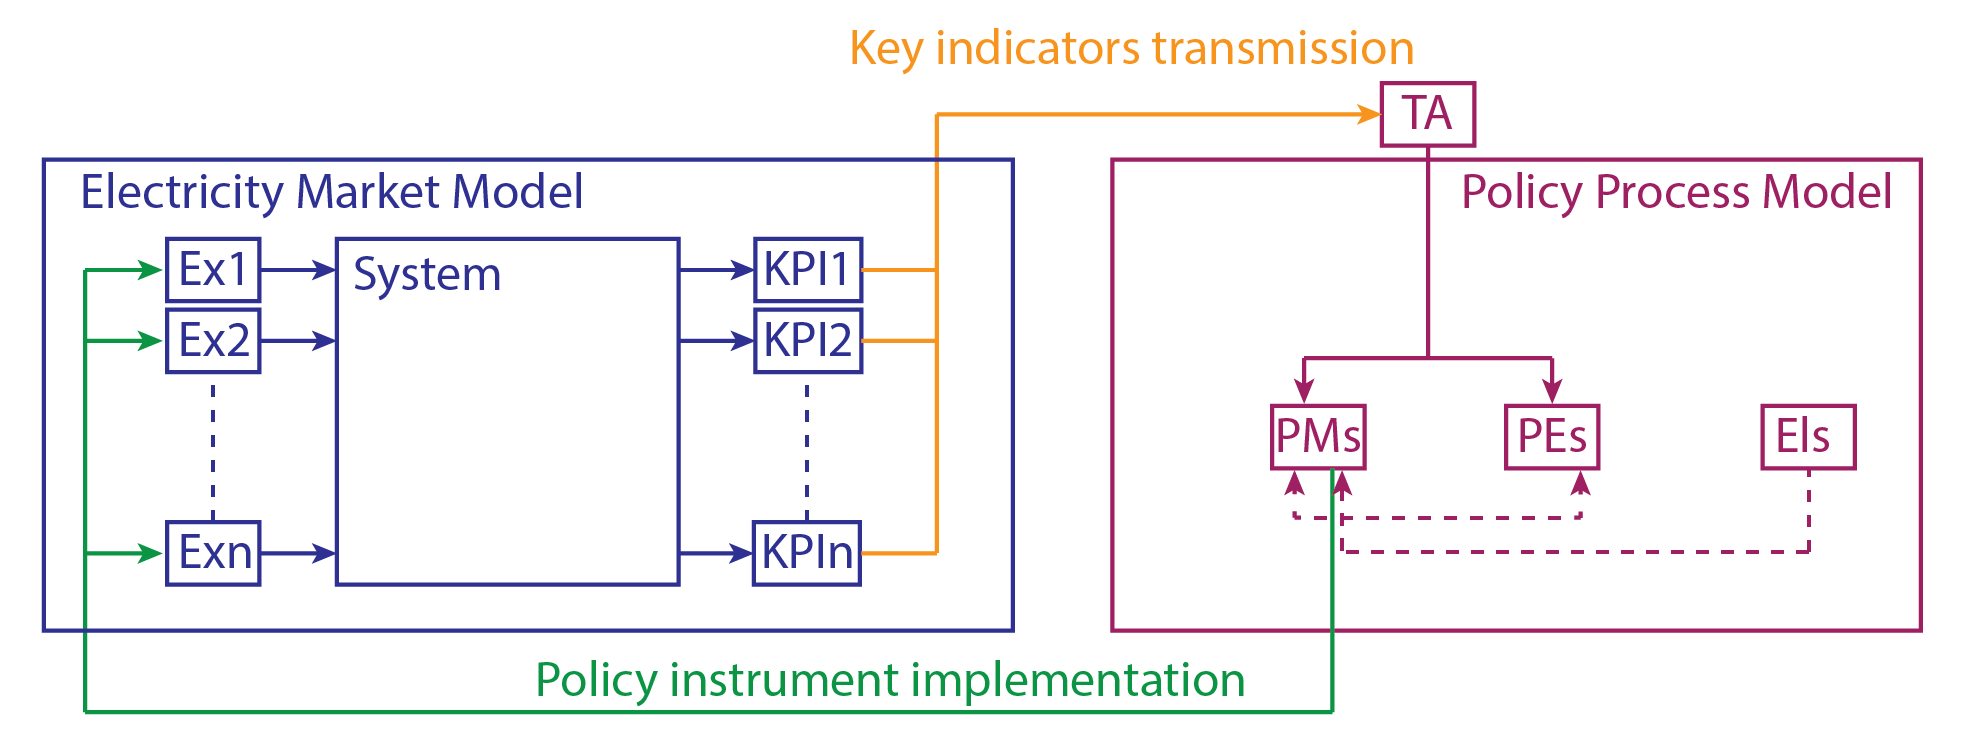
\includegraphics[width=\linewidth, keepaspectratio]{figures/ModuleInterface-09}
\caption{Diagram of the hybrid model.}
\label{fig:ModuleInterface-09}
\end{figure}

%%%%%%%%%%%% end of subsection

%%%%%%%%%%%%
\subsection{The problem tree}
\label{ssec:interfaceProblemTree}

To couple the models, the agents in the policy process need to be provided with a problem tree. This problem tree is specific to the electricity market model as it is informed by the key performance indicators from that model. This was highlighted in the previous section. Beyond this, the problems selected are also informed from previous work done by \cite{markard2016socio}. They identified a number of problems (they call these beliefs in their publication) that are specific to the Swiss context. These are however limited to the deep core and policy core levels. Secondary problems are not included or researched and are therefore taken from the model only.

The difficulty in the creation of the problem tree is to associate the right indicators to the right problems. The first step is to not consider the deep core problems. These are considered to be normative problems. They are beyond the boundaries of the model, out of the scope. They are not a crucial aspect of the process as it is focused on policy core problems so it does not make a big difference if deep core problems are considered or not. The next step is to consider the secondary problems. These can be found directly within the model. They are indicators that are made into secondary problems. Not all indicators are considered, only a few are selected. These are considered to be the important ones for the agents in the policy process. Finally, there is the selection of the policy core problems. These are, in general, aggregates of the secondary problems. They are calculated as a function of the main model indicators.

For the policy core problems, there is an additional aspect that needs to be considered. In work performed by \citeauthor{markard2016socio}, policy core problems within the Swiss electricity market subsystem were identified. These are: seriousness of the problem, role of the state, environment, economy and society. Several of these cannot be obtained from the model as they are outside of the boundaries of the model. However, the environment and economy can be considered. They are therefore selected as the policy core problems. \cite{markard2016socio} also identified four secondary problems. They are however not suitable for the model as they are more questions than problems. Furthermore, four secondary problems is not sufficient. It is for this reason that the secondary problems are only selected from the model. Ultimately, the policy core problems are calculated using linear equations that include a number of the indicators used for the secondary problems.

Overall, the problem tree is given as follows:

\begin{itemize}
\item Policy core problems:
	\begin{itemize}
	\item Economy
	\item Environment
	\end{itemize}
\item Secondary problems:
	\begin{itemize}
	\item Renewable energy production
	\item Electricity prices
	\item Renewable energy investments
	\item Domestic level emissions
	\item Imported emissions
	\end{itemize}
\end{itemize}

The economy takes into account elements related to profits of firms along with the security of supply of the country. The environment takes into account aspects such as the emissions, the amount of renewable energy and the amount of imported emissions.

%From markard2016socio, no deep core beliefs. Policy core beliefs are: seriousness of the problem, role of the state, environment, economy and society. In total, they identified 18 policy core beliefs. Most of these are beyond the scope of the model. The secondary beliefs identified are: phase out of nuclear, new nuclear plants, expansion of RES targets, expansion of energy demand targets, electricity suppliers role to fulfil efficiency targets.

%\begin{itemize}
%\item DC0 - Economy
%\item DC1 - Ecology
%\item PC0 - Security of supply
%\item PC1 - Profit levels - This is the average profits divided by the average revenues
%\item PC2 - Emissions - This is the average of domestic and imported emissions.
%\item S0 - Renewable energy production - This is calculated as the amount of renewable energy produced locally divided by the amount of energy produced overall.
%\item S1 - Nuclear production - This is the average production of nuclear over the total domestic production.
%\item S2 - Fossil fuel production - This is the average production of gas over the total domestic electricity production.
%\item S3 - Amount of imports
%\item S4 - Amount of exports - This is the average total amount of exports divided by the total demand
%\item S5 - Electricity prices - This is the price average. A maximum average price of 100 is assumed.
%\item S6 - Investment levels - This is the amount of investment (renovation + construction spent) over the amount of 
%\item S7 - Imported emission levels - This is the sum of all imported emissions from fossil fuel power plants divided by the total imported electricity. A maximum has to be found for normalisation based on average values.
%\end{itemize}

%%%%%%%%%%%% end of subsection

%%%%%%%%%%%%
\subsection{The policy instruments}
\label{ssec:interfaceInstruments}

The policy instruments within the policy tree are implemented using incremental increases and decreases in the following exogenous parameters.

\begin{enumerate}
\item Solar subsidies [+/- 0.04]
\item Wind turbine permit times [+/- 0.04]
\item Agent's hurdle rate  [+/- 0.02]
\item Carbon tax on domestic fossil fuel [+/- 10]
\item Carbon tax on fossil fuel imports [+/- 10]
\end{enumerate}

%%%%%%%%%%%% end of subsection


%%%%%%%%%%%%%%%%%%%%%%%
\chapter{Implementation}
\section{The electricity model}
\label{sec:ImplementationElec}

This section outlines the different algorithms that are used within the electricity market model.

\textcolor{red}{Chapter missing key elements like the merit-order curve algorithm.}

%%%%%%%%%%%%%%%%%%%%%%%%%%%%%%%%%%%
\subsection{Electricity costs calculation per technology}

% notes:
% what is the difference between operational costs and marginal costs?
% opportunity costs considers the costs that would be gained by waiting and selling at another time

The calculation of the price at which each asset sells its electricity varies depending on the technology considered. The details of the calculations for the marginal costs are presented below:

\begin{itemize}

% solar
\item For solar power plants:
\begin{equation}
MC_{solar} = VC_{solar}
\end{equation}

where $MC$ are the marginal costs and $VC$ are the variable costs.

% wind
\item For wind power plants:
\begin{equation}
MC_{wind} = VC_{wind}
\end{equation}

% hydro and hydro-p
\item For hydro and hydro-pumping power plants:
\begin{equation}
MC_{hydro} = OC + VC_{hydro}
% why 0.2?
\end{equation}

where $OC$ are the opportunity costs.

The opportunity costs are calculated using the price reference and depend on the amount of water that is left in the reservoir of the hydro power plant. The price reference is calculated based on the weighted average of the previous three year electricity price on the spot market in the previous years.

\begin{equation}
P_{ref} = 2 \cdot \frac{3\cdot P_{t-1} + 2\cdot P_{t-2} + P_{t-3}}{6}
\end{equation}

where $P$ is the average price of electricity on a given year and $t$ is the year within which the simulation is.

If the installed capacity is larger than the water left in the reservoir then, the opportunity costs are:

\begin{equation}
OC = (P_{ref} - VC_{hydro}) \cdot \left(1 - \frac{RL}{2 \cdot RC_{max}}\right)
\end{equation}

If the opposite is true, then:

\begin{equation}
OC = (P_{ref}  - VC_{hydro}) \cdot \left(1 - \frac{RL - IC}{RC_{max}}\right)
\end{equation}

where $RL$ is the reservoir level, $IC$ is the installed capacity and $RC$ is the reservoir capacity

% run of river
\item For run of river plants:
\begin{equation}
MC_{ror} = VC_{ror}
\end{equation}

% waste power plants
\item For waste management power plants:
\begin{equation}
MC_{waste} = OC_{waste}
\end{equation}

Here the costs are calculated using the opportunity costs again. These can be found using the same equations as for hydro power plants.

% thermal power plants
\item For thermal power plants:
\begin{equation}
MC_{thermal} = FC + VC_{thermal}
\end{equation}

where $FC$ are the fuel costs. The fuel costs include both the gas price and the carbon price. This considers a price for carbon that varies over time and emissions of 0.342834 tons/MWh (NREL, 2018).

Below is the carbon prices scenario:

\begin{center}
\begin{tabular}{ |c|c| } 
\hline
2017		& 9 \\ \hline
2020		& 15  \\ \hline
2025		& 22  \\ \hline
2030		& 33  \\ \hline
2035		& 42 \\ \hline
2050		& 73 \\
 \hline
\end{tabular}
\end{center}


% nuclear power plants
\item For nuclear power plants:
\begin{equation}
MC_{nuclear} = FC + VC_{nuclear}
\end{equation}

\end{itemize}

%%%%%%%%%%%%%%%%%%%%%%%%%%%%%%%%%%%
\subsection{Supply amount per technology}

The amount of electricity supplied per technology is given using the following equations:

\begin{itemize}

% solar
\item For solar power plants:
\begin{equation}
S_{solar} = C \cdot Solar_{conditions} * UF
\end{equation}

where $S$ is the supply, $Solar_{conditions}$ is an input file defining how much solar electricity was produced for every hour of the year historically, $UF$ is the potential utilisation factor. The potential utilisation factor is calculated based on a curve that helps assess the best locations for solar and the maximum theoretical amount of roof top solar in Switzerland. The curve is given below:

\begin{center}
\begin{tabular}{ |c|c| } 
\hline
0		& 0.147 \\ \hline
0.0367	& 0.1358  \\ \hline
0.9306	& 0.114155  \\ \hline
1		& 0.100114  \\
 \hline
\end{tabular}
\end{center}

% wind
\item For wind power plants:
\begin{equation}
S_{wind} = C \cdot Wind_{conditions} * UF
\end{equation}
where $Wind_{conditions}$ is an input file defining how much solar electricity was produced for every hour of the year historically, $UF$ is the potential utilisation factor. The potential utilisation factor is calculated based on a curve that helps assess the best locations for wind and the maximum theoretical amount of wind power in Switzerland. The curve is given below:

\begin{center}
\begin{tabular}{ |c|c| } 
\hline
0		& 0.3196 \\ \hline
0.181	& 0.2497  \\ \hline
0.195	& 0.2457  \\ \hline
0.267	& 0.2301  \\ \hline
1		& 0.1608 \\ 
 \hline
\end{tabular}
\end{center}

% hydro and hydro-p and waste
\item For hydro, hydro-pumping and waste power plants:

The supply of electricity is dependent on the level of the reservoir. If the reservoir level is below the capacity of the power plant, then the reservoir level is the amount supplied, otherwise, the capacity of the power plant is the electricity supplied.


% run of river
\item For run of river power plants:

\begin{equation}
S_{ror} = flow_{ror} \cdot growth_{ror} \cdot C_{ror}
\end{equation}

where $C$ is the installed capacity and the flow is dependent on weather input data.

The run of river growth factor represents the growth of such production over the year. It is based on a scenario provided in \autoref{tab:RORgrowthFactor} and can be calculated using the following equation:

\begin{equation}
growth_{ror} = C_{ror,scenario}/C_{ror,installed}
\end{equation}

This considers the entire run of river production within Switzerland and not just one plant.

\begin{table}[h!]
\begin{center}
\begin{tabular}{ |c|c| } 
\hline
2015		& 16400 \\ \hline
2020		& 16700  \\ \hline
2025		& 16933  \\ \hline
2035		& 17533  \\ \hline
2050		& 18333 \\ 
 \hline
\end{tabular}
\end{center}
\caption{Expected total production for all run of river power plants in GWh.}
\label{tab:RORgrowthFactor}
\end{table}

% thermal
\item For thermal power plants:
\begin{equation}
S_{thermal} = C
\end{equation}

% nuclear
\item For nuclear power plants:
\begin{equation}
S_{nuclear} = C
\end{equation}

Note that nuclear power plants are not online throughout the year. They have a yearly planned maintenance, usually planned in the summer when the plant is offline. This is a done over a period of thirty days. Each starting month is specified as an input per asset.

\end{itemize}

%%%%%%%%%%%%%%%%%
%\subsection{Spot market algorithm}
%\label{ssec:elecSpotMarket}

%%%%%%%%%%%%%%%%
\subsection{Investment approach}
\label{ssec:elecInvestments}

The electricity price forecast is used for the investments. This price forecasts consists of estimating a linear relation for the future in the form $y = mx + p$.

The slope $m$ is calculated using the following equation:

\begin{equation}
U = \frac{P_{t-0} + P_{t-1} + P_{t-2} + P_{t-3}}{4}
\end{equation}

\begin{equation}
m = \frac{- 3 \cdot \left(P_{t-3} - U \right) -  \left(P_{t-2} - U \right) + \left(P_{t-1} -  U \right) + 3 \cdot \left (P_{t-0} -  U \right)}{2 \cdot 2015}
\end{equation}

The constant $p$ is given by:
\begin{equation}
p = U - t * m
\end{equation}

where $t$ is the time at which the simulation is at.

The profitability of an asset is calculated using the following equation:

\begin{equation}
P = \left( \sum^t \frac{((Y+t) \cdot m + p) - VC}{(1 + r)^{t+1}} \right) \cdot 8760 \cdot \epsilon \cdot C
\end{equation}

where $P$ are the profits, $Y$ is the initial year, $t$ the year for which profitability is considered after the initial year, $VC$ the variable costs, $r$ the discount rate, $\epsilon$ the utilisation rate and $C$ the capacity of the asset considered.

The losses are calculated using:
\begin{equation}
L = \left( \sum^t \left[1 + \frac{1}{(1 + r)^{t+1}} \right] \right) \cdot FC \cdot C
\end{equation}

where $L$ are the losses, $C$ is the capacity of the plant and $FC$ are the annual fixed costs of the plant.

The profitability is then calculated as the difference between profits and losses.

For investments, the actors use the NPV and the profitability index of potential new power plants. 

The following equations are used to estimate the NPV.

\begin{equation}
NPV = \sum_{n=0}^N \frac{C_n}{(1+r)^n} = \sum_{n=0}^{N} \frac{(R-MC)*\epsilon-OC}{(1+WACC)^n}
\end{equation}

where $R$ are the revenues per year, $\epsilon$ is the utilisation factor, $MC$ are the marginal costs, $OC$ are the fixed operating costs. WACC is given as the sum of the risk rate and the discount rate.

%%%%%%%%%%%%%%%% end of the subsection


%\section{The policy process model}
\label{sec:ImplementationPolicy}

Due to the iterative process and after a reflection period, several parts of the formalisation was modified. This was done after the code had been implemented, it is therefore not mentioned in the main body of this report. The changes considered are presented here with a full rewrite of the formalisation.

% THE COMMON CORE
\section{Common core}

The common core is the centre part of the model which contains the concepts that can be placed in common for all policy making theories. The different parts of the common core are addressed here in the same order as they were addressed in the conceptualisation in \autoref{cha:conceptualisation}.

%- PARAMETERS - The system and subsystems	
\subsection{The subsystems}

The policy arena is designed as a subsystem in this formalisation. This term is borrowed from the advocacy coalition framework and represents the arena in which all the actors interact and influence on another. Each subsystem contains the different rounds: agenda setting, policy formulation and world.

%- PARAMETERS - The agents
\subsection{The agents}

The model is composed of five types of permanent agents and one temporary agent. These are divided in two main categories: the agents considered as they have to spend resources to perform actions and the agents that are passive as all the actions they perform happen regardless of resources or of the situation. One agent fits in both categories.

%0
\paragraph{Active agents}

The active agents are the policy makers, the policy entrepreneurs and the external parties. Note that the external parties also have a passive role in which they provide the states from the truth agent, to the policy makers, the policy entrepreneurs and the electorate. This is considered to be a passive action as it is independent of resources.

The active agent's attributes are given as follows:

\begin{enumerate}

\item The \emph{active agent} is represented as an 10-tuple given by \texttt{agent = (ID, subsystem, type, beliefHierarchy, affiliation, advocacy, resources, coalition, team, networkStrategy)} where
\texttt{ID} is the unique ID of the agent,
\texttt{subsystem} is the subsystem ID in which the agent is present,  
\texttt{type} is the choice of agent type, 
\texttt{beliefHierarchy} is the agent's personalised belief hierarchy, 
\texttt{affiliation} is the political entity the agent identifies with,  
\texttt{advocacy} is the list of the issues the agent is supporting, 
\texttt{resources} is the agent's resources (a relative value), 
\texttt{coalition} is the coalition ID to which the agent is a member of, and 
\texttt{team} is the team ID to which the agent is a member of,
\texttt{networkStrategy} is the strategy that the agent will use for his/her networking actions.

\item A \emph{type} corresponds to a choice of agent. This can either be a policy maker, a policy entrepreneur or an external party. Depending on the type of agent, the actions will change from one agent to another.

\item The \emph{belief hierarchy} is made of two main parts: the agent's own belief hierarchy structure and associated values, and the belief hierarchies of all other agents and their values based on the agent's perceived knowledge of their beliefs (also referred as partial knowledge). The entire \emph{belief hierarchy} structure is therefore a list of belief hierarchies which is as long as the number of agents present in the model. The details of the hierarchy structure itself are provided later on.

\item The \emph{advocacy} is represented as a 4-tuple \texttt{(prob\_as, pol\_as, prob\_pf, prob\_as)} where \texttt{prob\_pf} is the problem chosen by the agent during the agenda setting process, \texttt{pol\_as} is the policy chosen by the agent during the agenda setting process, similarly \texttt{prob\_pf} and \texttt{pol\_pf} are the problem and policy selected by the agent during the policy formulation process. Note that some of these might not be used depending on the theories considered at any point. For the common core, only the problem is used.

\item The \emph{resources} are represented as a decimal on the interval [0, 1]. Resources are distributed to the agents based on their affiliation and on that affiliation's representation within the model. These resources are used by the agent to perform actions on other agents. The resources are relative amongst all agents.

\item The \emph{team} is represented as a 3-tuple given by \texttt{(team ID, belonging, strategy)} where \texttt{team ID} is the team to which the agent belongs, \texttt{belonging} is the agent’s feeling of belonging in a team and \texttt{strategy} is the agent's strategy when wanting to create a new team.  This attribute is only used in the three streams theory. The \emph{belonging} value relates to how much the agent feel (s)he is part of a team and defines the amount of resources the agent is willing to commit to his team. The \emph{strategies} refers to the strategy selected by the modeller for an agent when it comes to the creation of a team.

\item The \emph{coalition} is represented as a 2-tuple given by \texttt{(coalition ID, belonging)} where \texttt{coalition ID} is the coalition to which the agent belongs and \texttt{belonging} is the agent’s feeling of belonging in the coalition.

\end{enumerate}

%0
\paragraph{Passive agents}

The passive agents are the truth agent and the electorate. Both types of agents only perform passive actions.

\emph{The truth agent: } The truth agent is an agent not mentioned in the conceptualisation but required for the formalisation. This agent helps make the link between the world and the agents within the model. It gathers all the states of the world and provides them, as they are, to the external parties. One truth agent is present per subsystem. The only attribute of the truth agent is the belief hierarchy. This is a different one that for the active agents. It only contains the overall similar structure without any causal relations. Furthermore, it only contains the states for each of the issues.

\emph{The electorate: } The electorate represents the different constituencies within a subsystem. There are as many electorate agents as there are political affiliations in the model per subsystem. The role of the electorate is to influence the policy makers in their aims. The following defines the attributes of the electorate.

The \emph{electorate} can be given as a 6-tuple written as: \texttt{electorate = (ID, subsystem, affiliation, beliefHierarchy, representation)} where \texttt{ID} is the unique name of the electorate, \texttt{subsystem} considers in which subsystem it is, \texttt{affiliation} is its associated affiliation, \texttt{beliefHierarchy} is the associated belief hierarchy of the electorate and \texttt{representation} is the percentage of the total population which this electorate represents within the model. The sum of all \emph{representation} from all electorates must always be equal to 100. The \texttt{representation} parameter affects the amount of resources received by the agents in the model. The belief hierarchy of the electorate is similar in structure to the one of the truth agent. It only contains the issues.

%- PARAMETERS - The belief hierarchy
\subsection{Belief hierarchy}

The belief hierarchy is composed of two main parts: the issues and the causal relations. The issues are categorised in multiple layers: the deep core issues (the top layer), the policy core issues (the middle layers) and the secondary issues (the bottom layer). Secondary issues are linked to policy core issues through causal relations while policy core issues are linked to deep core beliefs through different causal relations. If multiple layers of policy core issues are present, each layer is also linked to each other with causal relations. The overall representation of this hierarchy structure is shown in \autoref{fig:Formalisation-04} for a three layered hierarchy.

Each issue is categorised by four parameters: the state, the aim, the preference and the awareness. The state defines the view of the agent of a certain issue as it is in the world. This view does not have to match reality and can be influenced by other agents. The aim shows what the agent would like to see happening in the world. The preference  which is a derived parameter, defines the urgency that the agent places on the each issues. It is calculated depending on the state of the issue, the aim of the agent and the causal relations linked to this issue. The sum of all preference weights on any single layer of the belief hierarchy have to be equal to 1. Finally, the awareness represents the fact that agents are aware of a specific issue or not. It can take the value of 0 or 1. If an agent is not aware of an issue, it will not consider it in any calculation as if it did not exist. The belief hierarchy structure also contains causal relations. These link the issues on the different layers of the structure. These are the representation, in the agent's mind, of how each of the issues are related to each other within the technical model and which issues affect which other issue.

\begin{figure}
\centering
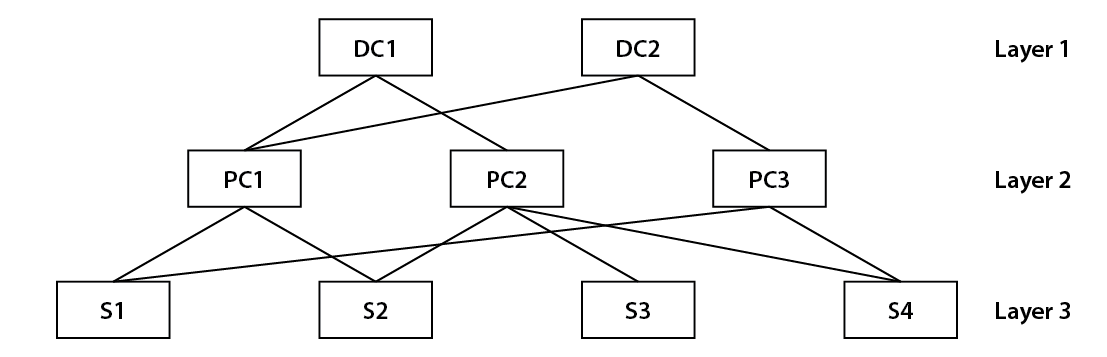
\includegraphics[scale = 0.75, angle = 0]{figures/Formalisation-04}
\caption{Example representation of a belief system with the three layers and several links between the layers. Not all possible causal relations are represented.}
\label{fig:Formalisation-04}
\end{figure}

Each agent has an attribute called \texttt{beliefHierarchy}. This attributes contains two parts as mentioned previously: the agent’s own belief hierarchy and the perceived hierarchies of all other agents in the model. It can be written as follows:

\begin{equation}
beliefHierarchy = [own_{hierarchy}, others_{hierarchy, n}]
\end{equation}

where $n$ represents the number of agents present in the model.

To further specify the hierarchy of the agent considered, the following can be said:

\begin{equation}\begin{split}
own_{hierarchy} &= [issues_k, causal\text{ }relations_l]\\
issues &= [state, aim, preference, awareness]
\end{split}\end{equation}

where $k$ defines the number of issues present in the belief hierarchy structure and $l$ the number of causal relations.

And it is also possible to specify the structure used to saved the perceived knowledge of the belief of the other agents:

\begin{equation}\begin{split}
other_{hierarchy} &= [issues_k, causal\text{ }relations_l]\\
issues &= [state, aim]
\end{split}\end{equation}

In both cases, the issues are specified with deep core issues first, policy cores following and ending with secondary issues. The causal relations are specified in the following example order: DC1-PC1, DC1-PC2, DC2-PC1, DC2-PC2, PC1-S1, PC1-S2, .... The state, preference and causal relation parameters are then specified on the interval of [-1, 1]. The preference is a percentage based parameters and is therefore calculated to be a number on the interval [0, 1].

%- PARAMETERS - The policy network
\subsection{Policy network}

The policy network is the network that links all agents within a subsystem. This network is composed of links with the following attributes: 

\begin{enumerate}
\item A \emph{policy network link} is represented as a 7-tuple \texttt{link = (agent1, agent2, awareness, awarenessDecay, conflictLevel)} where \texttt{agent1} and \texttt{agent2} are the agents at the end of a link, \texttt{awareness} is the awareness value, \texttt{awarenessDecay} is the decay value at which the awareness diminishes per time interval and \texttt{conflictLevel} is the conflict level characterising the relation between two agents for specific issues.

\item The \emph{awareness} value can take three main values. The value -1 refers to the fact that both agents are not aware of each other’s existence. They cannot network together without external introduction from a third party. For the value 0, the actors have no connection but know each other exist. They cannot network together until they have raised their awareness level to a non-negative value through networking actions. Any positive integer relates the value of awareness between the two agents. The awareness is given on the interval $]0,1]$. Note that awareness is relative amongst all links. The policy network links between policy makers can never be -1 as policy makers are public figures. Furthermore, a link cannot be downgraded to -1, it can only start at -1. As the awareness decays over time at a specific rate, there are several actions or events that can lead to a growth or stop the decay in the awareness between two agents. This is detailed later on.

\item The \emph{awareness decay} is represented by a 3-tuple \texttt{(value, time)} where \texttt{value} is the current value of the decay coefficient and \texttt{time} is a countdown. This countdown is by default set at 0, at which point decay of the awareness will happen. The countdown can be set at different values depending on actions that agents performed. The countdown will then go down to 0 every tick by 1. Whenever the countdown is not at 0, the decay is stopped.

\item The \emph{conflict level} parameter is determined for each agent for each issue's aim and state and for causal relations. Note that the conflict level between two agents will be difference depending on which agents is considered as the conflict level is obtained based on the perception of another agent's beliefs. The conflict level is therefore given as a 2-tuple for each link: \texttt{(agent 1, agent 2)}. Then for each agent, the conflict level is defined per issue for the state and then for the aim, and all causal relations. The conflict level is then calculated using:

\begin{equation}\begin{split}
CW \text{ }conflict \text{ } level_{n,n_m} &= |CW_n - CW_{n_m}| \\
aim \text{ } conflict \text{ } level_{n,n_m} &= |A_n - A_{n_m}| \\
state \text{ }conflict \text{ } level_{n,n_m} &= |S_n - S_{n_m}|
\end{split}\end{equation}

where $CW$ the causal weight, $A$ is the aim, $S$ is the state, $n$ is the agent for which the conflict level is calculated and $n_m$ is the perceived belief of agent $n$ on agent $m$ for that specific issue.

The resulting value is then formatted into a coefficient to be used in the grading of actions as is shown later on. When the result obtained is between 0 and 0.25, the conflict level is considered to be low, the coefficient is then set at 0.75. When the result obtained is between 0.25 and 1.75, the conflict level is considered to be medium, the coefficient is set to 0.85. Finally for a result higher than 1.75, the conflict level is considered high and the coefficient is set to 0.95. Note that both the intervals and the resulting coefficients can be varied by the modellers during experimentations to better tailor their model to their case studies.

\end{enumerate}

%-
\paragraph{Network upkeep and maintenance}

Each agent must maintain his/her policy network. For this, 20\% of agent’s resources can be used. The agents are allowed five actions, each time spending 4\% of the total amount of resources for each action. The order in which agents are selected to perform their network actions is random. These numbers can be changed by the modellers for the purpose of theirs cases.

Two strategies are differentiated for these actions. The modellers have to specified which strategy each agent uses in the model inputs. They are given as follows:

\begin{enumerate}
\item Largest network strategy - the agent will look into increasing his/her network as much possible:
	\begin{enumerate}
	\item The agent first wants to keep all links active. Any link that is below 30\% awareness level will be targeted for action. The lowest, but still above 0, will have priority.
	\item If all links are above 30\% awareness, the agent will look into introducing new links which had 0\% awareness. The priority is placed on the link with agents with the closest beliefs.
	\item If there are still resources left after step 1 and 2 are complete, the agent will maintain the links with the lowest awareness level in the network.
	\end{enumerate}

\item Focused network strategy - the agent will focus on maintaining a network of agents sharing its beliefs: (note that when it is stated similar belief, this relates to the problem that the agent is advocating for and no other issue)
	\begin{enumerate}
	\item The agent will look first for link where an agent with a similar belief (one of the agents has his belief within 0.2 of the other agent's aim belief) or higher belief level and with a awareness which is lower than 70\%. The agent will prioritise based only on the awareness level as long as the belief criteria is met.
	\item If no link qualifies, then the agent will seek to introduce new links in his/her network. The agent will select agents that have a similar belief or higher belief level.
	\item If both step 1 and 2 are met, the agent will look into maintaining an awareness level above 70\% for links still in service. The priority is put on the links with the lowest awareness value.
	\item If all previous steps are met, then the agent will simply look for new links with the priority placed on agents sharing his/her beliefs.
	\end{enumerate}
\end{enumerate}

The different actions mentioned above are performed as follows:

\begin{itemize}
\item An agent can increase the awareness in a network link if he feels the awareness level is too low. This awareness maintenance is dependent on three main parameters: the resources spent and the affiliation of both agents. The total increase in awareness for such an actions is calculated as:

\begin{equation}
awareness := awareness + resources \cdot affiCoef_{Aff_n,Aff_m}
\end{equation}

where the $affiCoef_{Aff_n,Aff_m}$ is the weight related to the affiliation of the two agents. If they share the same affiliation, then it is equal to 1.

\item Agents can also establish links with other agents for which they know they exist. This action can only be performed when the \texttt{link.awareness} parameter is equal to 0.

If this is the case, then the awareness can be increased through the spending of resources. The new awareness level is then calculated similarly to the awareness maintenance but with a small malus to account for the initial investment costs. The equation is given as follows:

\begin{equation}
awareness := resources \cdot affiCoef_{Aff_n,Aff_m} \cdot 0.5
\end{equation}

\item The notion of similar belief is defined as agents being close for the aim on issues at the policy core level. There are several steps to seek agents with similar beliefs:

\begin{enumerate}
\item Seek all links with awareness equal to 0 or higher and select their associated agents.
\item Select the aim parameter of the problem of the original agent.
\item For each associated agent, check its aim parameter for this same problem issue.
\item Calculate the difference of the parameter between the original agent and the associated agent for this issue.
\item Rank all differences from lowest to highest where the lowest is considered to be an agent of similar beliefs.
\end{enumerate}

This ranking is calculated based on the agent’s partial knowledge of other agent’s beliefs.
\end{itemize}

%- PARAMETERS - The affiliation network
\subsection{Affiliation network}

The affiliation network is a network that looks at the political affiliation of the different actors. Its links are represented as a 3-tuple given by \texttt{(affiliation1, affiliation2, affiCoef)} where \texttt{affiliation1} and \texttt{affiliation2} are the affiliations that are connected by the link and \texttt{affiCoef} represents the influence that an actor with an affiliation 1 can have on an actor with affiliation 2. The \emph{affiliation coefficient} is given on the interval $[0,1]$.

%- Actions
\subsection{The actions - Policy Makers}

There is a set of actions that policy maker agents can perform within the model. These actions are individual framing where the causal relations are the target of the influencing action, aim influence where the issue aim is the target of the influencing acton and state influence where the issue state is the target of the influencing action. These three times of actions are presented below in more details.

When selecting an action, the agent will perform all possible actions and calculate the likelihood grade of all actions. The agent will then select the action with the highest grade as the action to be implemented. The calculation of the likelihood of perfuming an action is mostly based on the beliefs of the influencing agent and his perception of the beliefs of the influenced agent. However, the actual impact of the action is based on the beliefs of the influencing agent and the beliefs of the influenced agent. This is an important difference that can sometimes justify why meaningless actions are performed. This can be due to a false perception of another agent’s beliefs.

%0
\paragraph{Individual framing}

The agents can attempt to influence the causal relation belief of other agents. This is an individual framing action. For this action, all causal relations related to the issue selected by the agent are considered. The likelihood to perform such an action depends on several parameters which are outlined below:

\begin{equation}\label{eq:likelihoodFraming}
G_{CW, n_m} = conflictLevel_{CW, n, m} \cdot affiCoef_{Aff_n,Aff_m} \cdot awareness_{n,m} \cdot actionWeight_{n,m}
\end{equation}

where $G$ stands for the grade, $n$ is the influencing agent, $m$ is the influenced agent. $n_m$ is the perfection of the beliefs of the influenced agent by the influencing agent and $CW$ is the causal weight of the causal relation

If this action is selected, as it has the highest grade, then the impact of the action on the beliefs of the influenced agents is given by:

\begin{equation}\label{eq:impactFraming}
CW_{m} := CW_{m} + \left(CW_{n} - CW_{m} \right) \cdot resources \cdot affiCoef_{Aff_n,Aff_m}
\end{equation}

%0
\paragraph{Individual action - Aim change}

The agents can also attempt to influence the aim beliefs on the different issues of the hierarchy of other agents. The likelihood that such action be performed is obtained in a similar way as shown below:

\begin{equation}\label{eq:likelihoodAimChange}
G_{A, n_m} = conflictLevel_{A, n, m} \cdot affiCoef_{Aff_n,Aff_m} \cdot awareness_{n,m} \cdot actionWeight_{n,m}
\end{equation}

The impact of such action is then calculated with:

\begin{equation}\label{eq:impactAimChange}
A_{m} := A_{m} + \left(A_{n} - A_{m} \right) \cdot resources \cdot affiCoef_{Aff_n,Aff_m}
\end{equation}

%0
\paragraph{Individual action - State change}

Similarly to the influence on the aims of an agent, the states can also be influenced. The likelihood of such an action being performed is given as follows:

\begin{equation}\label{eq:likelihoodStateChange}
G_{S, n_m} = conflictLevel_{S, n,m} \cdot affiCoef_{Aff_n,Aff_m} \cdot awareness_{n,m} \cdot actionWeight_{n,m}
\end{equation}

And the impact is calculated as follows:

\begin{equation}\label{eq:impactStateChange}
S_{m} := S_{m} + \left(S_{n} - S_{m} \right) \cdot resources \cdot affiCoef_{Aff_n,Aff_m}
\end{equation}

%0
\subsection{Preference calculation (issues)}

As mentioned earlier on, the policy maker has a limited attention span. This results in having to select one issue at a time for which (s)he thinks is the most urgent issue. This urgency is defined as the preference of an agent and is calculated for each layer in the belief hierarchy of the policy maker. Two cases must be distinguished for calculating this urgency: whether the layer considered is at the top or in the rest of the hierarchy. The preference is calculated for each issue and the sum of all preferences on each layer must be equal to 1.

\paragraph{Preference calculation for the principle beliefs}

For the top layer which is composed of the principle beliefs, the preference is calculated differently than for the other layers. This is because these beliefs are on the highest layer and can therefore not be connected to higher layers with causal relations. The calculation of the preference for each issue is given by:

\begin{equation}
P_i = \frac{ |A_i - S_i|}{\sum_{j=1}^n |A_j - S_j|}
\end{equation}

where $j$ is defined at the number of principle belief issues and $i$ characterises the principle belief issue being selected for the calculation.

\paragraph{Preference calculation for the policy core and secondary beliefs}

The preference calculation for the other layers in the belief hierarchy is adapted to include the causal relations that link these layers to higher up layers. This calculation applies to the policy core beliefs which are in the middle of the hierarchy and the secondary beliefs at the bottom.

To calculate the preference, the gap between aim and state for the issues is considered along with the impact of the causal relation on the gap of the issue on the above layers. The causal relations are not always helping bridge the gap between the aim and the state of issues on a higher layer. If this is the case, then the causal relations are not considered within the calculation as there effort is counter productive within the mind of the agent. The resulting equation that can be used to calculate the preference for these layers is given by:

\begin{equation}\label{eq:preference2}
P_k= \frac{ |A_k - S_k| + \sum_{j=1}^n |CW_j \left( A_j - S_j \right)|}{\sum_{l=1}^p \left[ |A_l - S_l| + \sum_{j=1}^n \left|CW_{j,l} \left( A_{j,l} - S_{j,l} \right) \right| \right]}
\end{equation}

The sums only include these terms if $CW_j$ and $\left( A_j - S_j \right)$ have the same sign. If it is not the case, these terms are not considered. And where $p$ is defined at the number of policy core issues, $k$ characterises the policy core issue being selected for the calculation, $j$ specifies the associated deep core and $CW$ represents the weight of the causal relation.

Based on these preferences obtained, the agent will select one issue to advocate for as mentioned earlier. For each layer, the agent will choose the issue with the highest preference. This is the case for each layer. The actions that the agent will then perform will be to influence other agents on the issue they have selected specifically.

%0
\subsection{Partial knowledge and awareness decay}

The likelihood of performing an action is based almost entirely on the perception of an agent on another agent’s beliefs. This is also referred as the partial knowledge of an agent. This partial knowledge is the representation that agents have of other agent’s beliefs. To perform better informed decisions, the agents must update their partial knowledge about other agents.

This update is performed after two agents have interacted with one another. When an action is performed, both agents have come into contact and have learnt about each other’s beliefs on the issue they have interacted on. This allows them to gain knowledge about the other’s belief. Therefore, for each action implemented, each agent will have access to the belief of the other agent concerning the issue influenced during the action. This access is not complete, the agents will gain the beliefs of the other agent with a small uncertainty amount.

Furthermore, because the two agents have interacted, their awareness of one another will not decline. It is therefore kept at the current level for several time steps. Only after these time steps have passed and if both agents have not interacted since, the decay of their awareness of one another will continue.

%- PARAMETERS - The agenda parameters	
\subsection{Agenda and agenda selection}

The \emph{agenda} is a 1-tuple given by \texttt{agenda = (issue, problem, policy)} where \texttt{issue} is the issue that is placed on the agenda by the policy makers, \texttt{problem} is the problem selected and \texttt{policy} is the policy selected by the policy makers. Note that the problem and policy attributes are only considered within the three streams theory, they are left empty within the common core.


To constitute the agenda, an issue has to be chosen for the entire subsystem. For this two methods are proposed which can yield different results. The first method considers all the top issues as graded by the policy makers. They are affected by their normalised resources. The grade of each issue is the sum of all agent's resources which have chosen that issue as their preferred issue. Whichever issue has the highest grade becomes the issue on the agenda.

The second method used for the ranking and selection of the issues is similar to the first one. The difference is that here all issues are taken from each policy maker. They are then weighed all together (and not simply the issues at the top of the ranking of each agent). This approach is meant to represent a different approach to the power dynamics in the model. The grade for each policy is then obtained as:

\begin{equation}
rankingGrade = \sum_{i=0}^n \left( \frac{1}{P_{rank}} \cdot resources_n \right)
\end{equation}

where $n$ is the number of agents and $P_{rank}$ is the ranking of the policy for that agent.

The issue with the highest grade is then taken as the issue for the agenda.

%- Actions
\subsection{The actions - Policy entrepreneurs}

The actions of the policy entrepreneurs are the same as the ones presented for the policy makers. The only difference is that the policy entrepreneurs cannot choose the agenda.

%- Actions
\subsection{The actions - External parties}

As mentioned in the conceptualisation, the have a more complex roles that the policy makers and entrepreneurs. They have different and similar actions to these actors. Their first role is to transmit the states of the world to the different agents in the model. This role is passive and does not require any resources. The second role is to blanket influence the electorates. For this 20\% of the resources of the external parties are used spent in interval of 10\%. The final role is an influencing role. Three actions are then available to the external parties: blanket framing, blanket aim influence and blanket state influence. 100\% of the resources are allocated for this actions to be spent in intervals of 10\%. For this all actions are graded and the one that is most likely to be considered is performed.

%0
\paragraph{Transmitting the states}

The states of the issue in the hierarchy beliefs of all agents are updated based on the information they get from the external parties. These external parties have access to the full and real states of the world. They can obtain these states from the truth agent which has the complete set of the states for each issue directly from the world. Each external party selects states that (s)he finds interesting to transmit them to other active agents. This transmission of the states can be affected by the political affiliation of the agents as agents of different affiliation are unlikely to fully trust one another. The equation used to calculate this update of the states is given below:

\begin{equation}
S_{agent} := S_{agent} + \frac{1}{n} \sum_{i=1}^n \left( \left(S_{EP_n} - S_{agent} \right) \cdot affiCoef_{Aff_n,Aff_m} \right)
\end{equation}

where $S$ stands for the issue state, $n$ is the number of external parties, $EP$ stands for external parties and $affiCoef_{Aff_n,Aff_m}$ is the affiliation related weight. The affiliation coefficient is the one that relates the affiliation of the agent and the affiliation of the external party selected. If an external party has not selected that specific state, then (s)he will not be able to provide the state for that issue. Furthermore, the external parties will only transmit the states to agents within their network. This can lead to some agents lacking states for specific issues because of the composition of their policy network.

%0
\paragraph{Electorate influence}

The external parties can also influence the goals of the electorate. This is done following the same template the goal influence of the policy makers and entrepreneurs. The only difference is that it is once again blanket influence which means that all electorate agents are affected at once. Note that because the external parties have a limited attention span, they can only influence the electorates on the issue they have selected. The impact of this influence is given by the following equation:

\begin{equation}
A_{El, i} := A_{El, i} + \left(A_{n, i} - A_{El, i} \right) \cdot affiCoef_n \cdot resources \cdot \frac{1}{nEl}
\end{equation}

where $n$ is the external party, $i$ is the issue and $nEl$ is the number of electorates.

%0
\paragraph{Blanket framing}

The external parties can also attempt to influence the understanding of the world of other external parties, the policy makers and policy entrepreneurs. The external parties perform such influence on all agents at the same time which leads to this action being called blanket framing. The overall calculation of the likelihood of performing such an action is similar to what was presented for the framing action of the policy makers. The impact is also similar but spread amongst all agents. Such action can only happen on the agents that are within the policy network of the external party. All causal relations related to the issue selected by the external party can be influenced.

The likelihood of performing a blanket framing action is calculated as follows:

\begin{equation}\label{eq:likelihoodBlanketFraming}\begin{split}
G_{CW, n_m} &= conflictLevel_{CW, n, m} \cdot affiCoef_{Aff_n,Aff_m} \cdot awareness_{n,m} \cdot actionWeight_{n,m}\\
G_{CW, n} &= \sum_{m = 1}^{nagents-1} G_{CW, n_m}
\end{split}\end{equation}

where $CW$ is the causal weight selected, $n$ the external party performing the framing, $m$ the affected agents considered and $nagents$ the total number of agents.

The impact of this action is then calculated for each agent using:

\begin{equation}\label{eq:impactBlanketFraming}
CW_{m} := CW_{m} + \left( CW_{n} - CW_{m} \right) \cdot resources \cdot affiCoef_{Aff_n,Aff_m} \cdot \frac{1}{nagents}
\end{equation}

%0
\paragraph{Blanket aim influence}

The external parties can also attempt to influence the aims of the other agents. This is done on all agents at once similar to the blanket framing.

The likelihood of performing a blanket aim influence action is calculated as follows:

\begin{equation}\label{eq:likelihoodBlanketFraming}\begin{split}
G_{A, n_m} &= conflictLevel_{A, n, m} \cdot affiCoef_{Aff_n,Aff_m} \cdot awareness_{n,m} \cdot actionWeight_{n,m}\\
G_{A, n} &= \sum_{m = 1}^{nagents-1} G_{A, n_m}
\end{split}\end{equation}

where $A$ is the aim of the issue selected, $n$ the external party performing the framing, $m$ the affected agents considered and $nagents$ the total number of agents.

The impact of this action is then calculated for each agent using:

\begin{equation}\label{eq:impactBlanketFraming}
A_{m} := A_{m} + \left( A_{n} - A_{m} \right) \cdot resources \cdot affiCoef_{Aff_n,Aff_m} \cdot \frac{1}{nagents}
\end{equation}

%0
\paragraph{Blanket state influence}

Finally, the external parties can attempt to influence the states of the other agents. This is done on all agents at once similar to the blanket framing.

The likelihood of performing a blanket framing action is calculated as follows:

\begin{equation}\label{eq:likelihoodBlanketFraming}\begin{split}
G_{S, n_m} &= conflictLevel_{S, n, m} \cdot affiCoef_{Aff_n,Aff_m} \cdot awareness_{n,m} \cdot actionWeight_{n,m}\\
G_{S, n} &= \sum_{m = 1}^{nagents-1} G_{S, n_m}
\end{split}\end{equation}

where $S$ is the state of the issue selected, $n$ the external party performing the framing, $m$ the affected agents considered and $nagents$ the total number of agents.

The impact of this action is then calculated for each agent using:

\begin{equation}\label{eq:impactBlanketFraming}
S_{m} := S_{m} + \left( S_{n} - S_{m} \right) \cdot resources \cdot affiCoef_{Aff_n,Aff_m} \cdot \frac{1}{nagents}
\end{equation}



%-
\subsection{Electorate passive action on policy makers}

The policy makers are passively influenced by the electorate. Each electorate has a certain affiliation to which policy makers are also related. Each policy makers' issue aim will be influenced by their respective electorate. This happens as a passive effect where the issue aims of the policy makers slowly progress towards the issue aims of the electorate. The equation to calculate the change in the aim of the policy maker is given as follows:

\begin{equation}
A_{PM} := A_{PM} + \left(A_{El} - A_{PM} \right) \cdot 0.001 \cdot \left| A_{El} - S_{El} \right|
\end{equation}

where $El$ stands for electorate and $PM$ for policy maker. Note that this is only performed for the issues of the policy maker for agents with matching affiliations. Furthermore, the value 0.001 is arbitrary and can be changed by the modeller depending on the case study.

%- PARAMETERS -  The policy instruments
\subsection{Policy instruments}

The policy instruments are measures that can are chosen by the policy makers to impact the real world. Policy entrepreneurs and external parties can also influence the policy makers in their choices. To assess the different policy instruments, the different active agents assess the impact of these instruments on the secondary issues in their belief hierarchy. These instruments have an impact on the gap between the states and the aim of each of these issues. The policy instruments can be described as follows:

\begin{enumerate}
\item A \emph{policy instrument} is represented as a 7-tuple \texttt{(name, impact, change, layer, children, awareness, feedback)} where \texttt{impact} is related to the impact of the policy on a specific issue, \texttt{change} is the objective change expected in the world due to this policy, \texttt{layer} corresponds to the layer in the instrument hierarchy (when used), \texttt{children} corresponds to the instruments linked to the selected instrument in the instrument hierarchy, \texttt{awareness} is related to the availability of the policy for a specific agent and \texttt{feedback} is related to the expected model feedback from the implementation of the policy considered.

\item The \emph{impact} of a policy instrument is given as a 2-tuple: \texttt{(issue, impact)} where \texttt{issue} defines which of the secondary issues is affected and \texttt{impact} specifies by how much.

\item The \emph{change} due to a policy instrument is the subjective representation of the impact of the policy instrument. These are the actual changes that will occur in the world with the implementation of the instrument. They are defined by the modeller and are fully independent on the agents.

\item The \texttt{layer} and the \texttt{children} are both parameters that related to the three streams theory. They are therefore outlined in that section and are left empty for the common core.

\item The \emph{awareness} parameter defines whether a certain policy instrument is known in a specific subsystem. This parameter is related to the diffusion theory and is further outlined in the section dealing with the diffusion theory.

\item The \emph{feedback} parameter contains the feedback effects as defined by the modeller. This parameter is related to the feedback theory and is further explained in the feedback theory section.
\end{enumerate}

%-
\subsection{Preference calculation (instruments)}

Similarly to the agenda setting round, in the policy formulation round, the agents have a limited attention span. They can therefore only select one policy instrument at a time. The calculations used to select these instruments are slightly different than the ones in the agenda setting. They are shown below

%0
\paragraph{Preference calculation}

The preference calculation of the secondary issues within the context of a policy formulation rounds are tweaked from the calculation presented in the agenda setting round. The main reason is that for the policy formulation, the number of issues considered is narrowed down by what is on the agenda. The agents can therefore only consider issues in the secondary belief layer that have a direct effect, according to their beliefs, on the issue that is on the agenda. All other issues are not included within the preference calculation. For the rest, \autoref{eq:preference2} is still used to calculate the preferences of the different issues for each agent according to their own beliefs.

%0
\paragraph{Instrument selection calculation}

Once the preferences for the different secondary issues have been attributed, it is possible to look at the preference of the instruments. These are used by the agents to assess the instruments and select the one they find most important. The equation that is used to calculate the preference of the different instruments is provided below. Similarly to the calculation of the preferences in the belief hierarchy, only instruments with impacts that have the same sign as the belief gap (aim minus state for a specific issue) are considered. The other instruments are counter productive and are therefore directly excluded from considerations.

\begin{equation}
P_i = \sum_{j=1}^n \left[ impact_j \cdot \left( A_j - S_j \right) \cdot P_j \right]
\end{equation}

where $n$ is the number of impacts this policy instrument has, and $j$ represents the secondary issue and the associated impact of the policy instrument on that issue.

Once all the preferences have been calculated, the agent will select the instrument with the highest preference. This will help define the actions that each agent can perform. Because no actions can be performed on the instruments directly, the agent will be able to perform actions on all issues directly related to the instrument and all causal relations which link the issue on the agenda and the issues related to this instrument. The likelihood and the impact of the actions are calculated in the same way as was shown previously. The aim here for the agents is to convince other agents that the instrument’s impact is as high as they perceive because their causal relations, aims and states beliefs are similar.

%-
\subsection{Policy instrument selection and implementation}

Similarly to the agenda setting round, the policy makers are the agents that can selected a policy instrument. Additionally, they will decide if a policy instrument should be implemented. This is done through one of two strategies which can be chosen by the modeller and which rare presented below.

%0
\paragraph{Unanimity}

If unanimity is required, all policy makers must have selected the same policy instrument for it to be implemented. If this is not the case, the instrument will not be implemented and the round will close without a definitive output.

%0
\paragraph{Majority}

If a majority is required, 50\% plus one policy maker must select the policy instrument for it to be implemented. The resources of the different policy maker has no impact on this majority as it had in the agenda setting round. If a majority cannot be found, the policy instrument will not be implemented.

%-
\subsection{External events}

The external events that are considered are external events that affect the agents. External events that would affect the world such as a flood for a hydrological model are of no interest and considered out of scope of this report. However, the impact on the model such as a change in the electorate composition due to the flooding is of interest.

The following is a non-exhaustive list of potential external events which the modeller could use.

\begin{enumerate}
\item An election - this would create a change in the electorate representation parameter which would in turn lead to different resources allocation for the policy makers.
\item The introduction of a new issue - a new issue could be introduced to the system or to a subsystem. This would affect the knowledge parameter for an issue for all agents present in the model.
\item Resources shift - a shift in the resources distribution due to an external event could be modelled. The way the resources are attributed could be modified to simulate a crisis situation were resources are scarce. This could also be modelled as a reduction in the possibility of actions (increasing the amount of resources that is spent per action).
parameter would be changed.
\item Policy network shifts - change in the awareness parameter of specific network links.
\item Affiliation network shift - change in the affiliation coefficient parameter that defines the interaction possibilities between two different political affiliations
\end{enumerate}

%-
\subsection{The model cycle}

For this formalisation, it is assumed that the different rounds are performed consecutively. First the agenda setting rounds are performed, then the policy formulation rounds and finally the real world. A further assumption is to assume that there is only one round of each of these steps is performed. This leads to a 3-step model with an agenda setting step, a policy formulation step and a world simulation step. The agenda which is obtained at the end of the agenda setting helps defines what the agents will be interacting about within the policy formulation.

This has several consequences. The first one is that the beliefs hierarchy of the agents must be a three-layer hierarchy. At the top are the principle beliefs, then in the middle the policy core beliefs and at the bottom the secondary beliefs. Within the agenda setting, the agenda decide on an agenda issue from the second layer, the policy core issues. Within the policy formulation, the agents select instruments which are related to the third layer.

The steps used to mode this approach are then detailed as follows:

\begin{enumerate}
\item World round:
	
	\begin{enumerate}
	\item \emph{World simulation:} The world which is an exogenous party to the model or an internal technical model are run to provide inputs for the next step.
	\item \emph{Trigger of external events:} Any event that the modeller decides to implement are activated at this stage of the model cycle.
	\item \emph{Update of the truth agent:} The technical output is converted into normalised data fitting with the issues present in the belief tree. These are placed in the truth agent's $S$ parameters.
	\item \emph{Electorate action on policy makers}
	\item \emph{Transmission of the states:} The external parties select their states of interest from the truth agent and pass the information to the agents within their policy network.
	\end{enumerate}
	
\item Agenda setting round:


	\begin{enumerate}
	\item \emph{Preference calculation (issues):} Each agent calculates the preference for their principle and policy core beliefs. The agents then each select an issue that (s)he will advocate for in his/her policy core beliefs based on the preferences calculated.
	\item \emph{Agent interactions:} 

		\begin{enumerate}
		\item \emph{Resources received:} Each active agent receives its resources based on his/her political affiliation.
		\item \emph{Network upkeep or maintenance}
		\item \emph{Belief influence actions:} All active agents perform their respective actions. The order in which the agents perform their actions is made random to not favour agents with first or last actions.
		\end{enumerate}

	\item \emph{Preference calculation (issues):} Each policy maker updates his preferences for his principle and policy core beliefs. This update of the preference is necessary to take into account the changes that might have occurred as a results of the agent interactions. Each policy makers choose the issue with the highest preference as their issue of preference.
	\item \emph{Agenda selection}
	\end{enumerate}
	
\item Policy formulation round:

	\begin{enumerate}
	\item \emph{Preference calculation (instruments):} Each agent update his preference for his secondary beliefs based on the issue on the agenda. Each agent then selects a policy instrument that (s)he will be advocating for.
	\item \emph{Agent interactions:} 

		\begin{enumerate}
		\item \emph{Resources received}
		\item \emph{Network upkeep or maintenance}
		\item \emph{Belief influence actions}
		\end{enumerate}

	\item \emph{Preference calculation (instruments):} Each policy maker upgrades their policy instrument preferences after the interaction step.
	\item \emph{Policy instrument implementation} 
	\end{enumerate}
	
\item \emph{The model advances:} The clock is advanced to the next tick. Programming of ticks actions are also performed (data collection, policy network awareness decay, …).

\end{enumerate}

% THE THREE STREAMS THEORY
\section{Three streams theory}

The three streams theory introduces a number of changes and additional concepts to the common core. These are detailed here. The first important addition and change is related to the policy instruments which are now assembled in an instrument hierarchy. Another change comes with the fact that the agent now must choose between a policy and a problem based on the calculated preference. Furthermore, because agents are not able to select policies, they are provided with an additional action. Finally, the agents can assemble in teams. This requires an algorithm for the creation of such teams and it brings in more actions that the actions can perform within and outside of their teams.

%-
\subsection{The policy instruments}

As explained in the conceptualisation, the actors now each have an instrument hierarchy similar to their belief hierarchy. To formalise this hierarchy, two attribute within the policy instruments are activated. These are the layer and children attributes. The layer attribute defines in which layer of the hierarchy the instrument fits. These layers are related to the layers present in the belief hierarch. This means that policy instruments in the second layer of the instrument hierarchy will have an impact on the issues which are in the second layer of the belief hierarchy. The children attributes helps understand which instruments are related across the different layers. This is defined by the modeller and is useful to navigate from one round to another. When a certain instrument is placed on the agenda from the second layer, then only his children present in the third layer can be considered by the agents. All other instruments are considered irrelevant. A representation of the instrument hierarchy is given in \autoref{fig:Formalisation-09}.

\begin{figure}
\centering
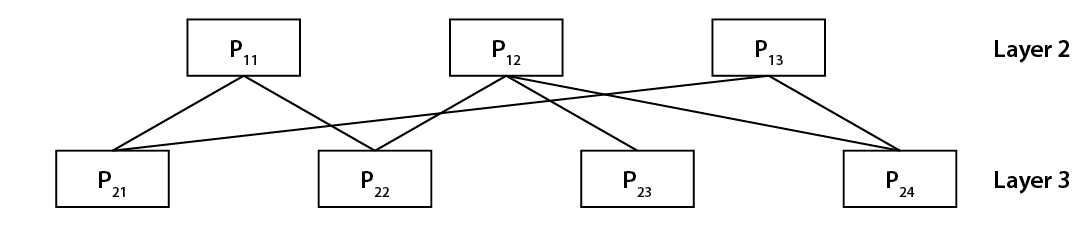
\includegraphics[scale = 0.75, angle = 0]{figures/Formalisation-09}
\caption{Instrument hierarchy representation with the two layers.}
\label{fig:Formalisation-09}
\end{figure}

There is an additional change that occurs within the policy instruments. The impact is not objective anymore. The impact is now a subjective parameters very much like the states and aims for the issues in the belief hierarchy. This is important as the agents will be able to influence other agents on their beliefs of the impact of the different instrument available to them.

%-
\subsection{Preference calculation (problems and policies)}

As mentioned within the conceptualisation, the agents can now select a policy or a problem. For that they must grade all problems and policies in every layer. They can then select the policy or problem that has the highest grade.

%0
\paragraph{Problem and policy preference calculation}

The problems and policy grades are obtained differently. The problems are based in the belief hierarchy and their grades are calculated similarly to the issues in the common core. The equation is given as:

\begin{equation}
G_{prob, i} = \left( A_i - S_i \right) + \sum_{j=1}^n \left| CW_j \left( A_j - S_j \right) \right|
\end{equation}

where $i$ corresponds to the policy core considered and $j$ the related deep core issues.

The policy instrument are assessed on their impact on the different gaps in their associated issues in the belief hierarchy. The equation used to calculate their grades is given by:

\begin{equation}
G_{policy, i} = \sum_{i=1} \left( A_i - S_i \cdot I_i \right)
\end{equation}

where $i$ corresponds to the policy core affect by the policy selected and $I$ is the impact expected from the policy.

Once all possible policies and problems have been graded, the agent will select the one with the highest grade. Then the process is repeated again but for the associated issues. This is done with only problems related to the policy selected if a policy was selected first or with the policies related to the problem selected if the problem was selected first.

The actions that the agents will perform will be based on whether they first selected a problem or a policy. These actions are detailed in a subsequent section.

%0
\paragraph{Agenda and agenda selection}

Within the three streams approach, the agenda selection is a little different than for the common core. The agenda is now composed of two parts: a problem and a policy. The issue attribute of the agenda is left empty. The rest is similar to the common. The problem selected for the agenda is the most popular problem for all agents considering their respective resources while the policy chosen is the most popular policy amongst all agents also considering their resources.

%0
\paragraph{Policy instrument selection and implementation}

For the policy formulation round, the procedure to select and implement a policy instrument is similar to the common core procedure. The policy chosen by all policy makers is considered. If a policy is beyond the threshold set but the modeller for implementation, the policy will be implemented. The problem chosen by the policy makers is not taken into account.

%-
\subsection{The actions (active agents)}

The influencing actions that the agents can perform are mostly similar to the ones in the common core. The main difference is that all their actions are performed on the problems if they have first selected a problem. The policy makers and entrepreneurs can perform framing, state influence and aim influence actions on other agents based on the problem they have selected in their belief hierarchy. The external parties can perform their blanket framing on other agents and blanket aim influence on the electorate. This is also based on the problem they have each selected.

For the agents that have selected a policy, an additional action is added. This action is an action that influences the impact beliefs of the policy instrument selected by the agent. For all agent, this action replaces the framing or blanket framing action. The aim and state influence actions remain the same. The likelihood of performing each action is calculated. Whichever action is most likely to be performed is implemented with a certain calculated impact.

The likelihood of performing a policy action is given as follows:

\begin{equation}\label{eq:likelihoodImpact}
G_{I_{issue}, n_m} = conflictLevel_{I_{issue}, n, m} \cdot affiCoef_{Aff_n,Aff_m} \cdot awareness_{n,m} \cdot actionWeight_{n,m}
\end{equation}

where $n$ is the agent performing the action, $m$ is the agent on which the action is performed, $I$ stands for the impact that the action has on the mentioned issue. Note that if the instrument has an impact on four separate issues, then the agent will assess the likelihood of influencing each of the four impacts contained in that policy instrument.

The impact of the action is then given as follows:

\begin{equation}\label{eq:impactImpact}
I_{m, issue} := I_{m, issue} + \left( I_{n, issue} - I_{m, issue} \right) \cdot resources \cdot affiCoef_{Aff_n,Aff_m}
\end{equation}

where $n$ is the agent performing the action, $m$ is the agent on which the action is performed.


%-
\subsection{The teams}

As mentioned in the conceptualisation, the three streams theory includes the concept of teams. This concept is formalised within this section.
Teams contain a number of agents that feel they share their beliefs for a specific issue. A team is therefore given as a 6-tuple written as: \texttt{(team ID, lead, members, issue, creation, resources)} where \texttt{lead} is the leader of the team (the agent that created the team), \texttt{members} is the list of members that are part of the team, \texttt{issue} is the policy issue that the team is advocating for (policy or problem), \texttt{creation} is the time at which the team has been created and \texttt{resources} consists of the resources at the disposal of the team to perform actions. The resources are calculated as the sum of all the members belonging level.

%0
\paragraph{Agent-team actions}

The agent-team actions are all actions that each agent performs to either decide to join or create a team. It also consists of actions related to the disbanding of teams and the checking that the team requirements are still met. Each agent goes through all of these actions each tick. Each agent can only be part of one team at a time in the agenda setting process and one team in the policy formulation process. Note that all actives agents can be part of teams. The following list presents the different actions that are taken in chronological order in which they are performed in the model: start a team, join a team, leave a team, disband a team and calculate belonging level.

%0
\paragraph{Start a team}

An agent that wants to start a team has to consider different requirements. Two different cases have to be considered here: the case where the agent first chose a problem and the case where the agent first chose a policy.

If the agent first chose a problem then the first requirement is that for the secondary issue chosen, the gap between aim and state must be above a certain threshold. This threshold is 0.8 in general but can be set to 0.5 in cases where a change in the magnitude of the state from the previous tick is larger than 0.5 (in case of an external event). This must be the case for all agents if they want to join the team. The second requirement relates to the belief states. For the agenda setting, it is the causal relation between the deep core issue with the highest preference for the starting agent and the policy core issue selected as the problem. For the policy formulation, the causal relation selected is the one relating the problem on the agenda and the secondary issue selected as the problem by the agent. All agents that want to join the team must be within 0.5 of the value of the causal relation for the agent starting the team.

If the agent first choses a policy, then there is a small change in the requirements looked at. The agent still looks at the gap requirement. However the second requirement is now dependent on the impact that the policy has on the secondary issues selected as the problem by the agent that is starting the team. The impact on the associated problem should be within 0.5 for the other agents considered to enter the team.

If both of these requirements are met, then the agents qualifies to join the team. Note that for each agent contacted, the agent starting the team loses 2\% of his resources and the contacted agent loses 1\% of his resources. This is to justify the resources needed for the exchange of knowledge. Furthermore, the agent starting the team will initially assess the other agents based on his knowledge of their beliefs. This leads to the spending of resources. If his perception of the other agent's beliefs are not true, then the agent will not join the team but the resources will have been spent regardless. The resources are also used to gain some information on the beliefs of the other agents. Even though the other agents might not be interested, spending these resources allow the agent to gain knowledge of the beliefs of the other agent within a certain range. Through this exchange of knowledge the agent also provides his own beliefs to the agent being contacted.

The creation of the team requirements are then based on the strategy that the agent is using. Two strategies are considered. The first strategy consists of starting a team with all the agents found that meet the requirements mentioned earlier. The team will then be composed of the maximum number of agents possible. The second strategy consists of starting a team once a certain number of agents has been established to meet the aforementioned requirement.

Upon the creation of a team, all agents that are part of the team are added to the member list. The lead agent of the team is the agent that started the team. Each agent's belonging level is also calculated based on a weighted average of the beliefs of the team on the state of the issue advocated for. Joining a team will also lead to the half of the awareness decay in the links between the agents present in the team, effectively counting as an action.

%0
\paragraph{Join a team}

An agent can join a team if (s)he is not already part of a team. For this, the agent will check the same requirements as when creating a team (gap and causal relation/impact requirements). This is done for the issue of the team (s)he is approaching. For each team that the agent probes, 2\% of his resources are spent. If the requirements are met, then the agent will join the team and be added as a member of the team. The agent is allowed to spend 50\% of his resources for such a search. Once these resources have been depleted or all team have been considered, the agent moves on.

%0
\paragraph{Leave a team}

An agent can leave another team for one reason: because his belonging level is too low. The belonging parameter of the agent is checked every time period. If it descends below 30\% then the agent will automatically leave the team. If the team remaining has less than three agents, it will be disbanded right away. Note that the belonging parameter is updated based on the perception of an agent on another agent's beliefs (partial belief) without full knowledge. This will artificially increase the life of teams. 

%0
\paragraph{Disband a team}

As mentioned earlier, a team will be disbanded if the problem or policy advocated by the team does not match the problem or policy advocated by the lead agent. This can be due to the leader being influenced and having changed his/her preferences. This is checked every five time periods. The second reason for which a team will be disbanded is if the agents present in the team to not meet the team creation requirements anymore. This is also checked every five time periods.

%A team can be disbanded if the lead agent in the team changes his advocacy parameter for which the team was created. This is checked every time period. A team can also be disbanded if the thresholds creation criteria are not met. This is checked every five time periods.  For this, the lead agent checks whether the other agent's are within 0.2 of his beliefs for the advocated issue. If they are within that threshold, then the team will remain. This check does not costs resources and is based on the lead agent's perception of the knowledge of the other agents. It does not require a knowledge exchange.

%0
\paragraph{Belonging level setting}

The belonging level in a team is used to measure how much resources an agent is willing to contribute to the team resources and how much (s)he will keep for his own individual belief influence actions. This belonging level is entirely related to the problem or the policy being advocated by the team.

The belonging level is obtained differently depending on whether the team has selected an problem or a policy. For a problem, the belonging level is obtained through the problem that is being advocated by the entire team. The steps are shown below:

\begin{enumerate}
\item The weighted average of all agent’s belief on the state of the problem being advocated by the team of all agent is calculated using:
	\begin{equation}
	S_{prob, weighted} = \sum_{i=1}^n resources_n \cdot S_n
	\end{equation}

	Note that this weighted average might be difference for each agent as it is based on partial knowledge and not full knowledge. The belonging parameter will be affected by the perception of other agent's beliefs.

\item The belonging level is then calculated using the following equation:
	\begin{equation}
	Belonging = 1 - \left| S_{prob,agent} - S_{prob,weighted} \right|
	\end{equation}
\end{enumerate}

The belonging level in a team that is advocating for a policy is different. It is calculated using the impacts that the policy has on the different issues in the belief hierarchy. The belonging level of each agent is calculated as the difference between his/her own total belief and the average of the other agent’s total beliefs. The ‘total belief’ of each agent is calculated for the policy that is being advocated by the team according to the agent’s own beliefs as the sum sum of the absolute value of all impact that policy has. To estimate the total belief of other agents, agents have to rely on their partial knowledge. The steps are provided below:

\begin{enumerate}
\item The total belief of all agents is calculated:
	\begin{equation}
	TB_{pol, m} = \sum_{i=1}^p |I_{n_m, issue}|
	\end{equation}
	where $m$ is the agent being considered, $n$ the agent performing the estimation of the total belief and $p$ the number of impacts that the policy instrument has.

\item The average of the other agent’s total belief is calculated:
	\begin{equation}
	TB_{pol, avg} = \sum_{i=1}^p |TB_{pol,m}|
	\end{equation}

\item The belonging level is then calculated using the following equation:
	\begin{equation}
	Belonging = 1 - \left| TB_{pol,m} - TB_{pol, avg} \right|
	\end{equation}
\end{enumerate}

%-
\paragraph{Team belief actions}

Once the teams have been constituted, these teams must perform actions. These are the belief actions. There are two types of actions that the team can conduct. They can first perform intra-team actions to help the team get more consistent beliefs. They can also perform inter-team actions. In this case the aim is to convince other agents outside of the team that the belief of the team are more important. Each type of actions uses 50\% of the resources reserved for the team. These actions are performed in intervals of 10\% of the total amount of resources reserved. The resources available to team are equal to the sum of the belonging attributes for each of the members of the team.

\begin{itemize}

\item Intra-team actions:

There are four main intra-team actions: blanket framing on causal relations, blanket framing on policy instrument impact, direct influence on aim and direct influence on state beliefs. The aim for these actions is to help the entire team be a more coherent entity with agents having similar beliefs regarding the issues they advocate for. As each of the team is based on awareness between the different agents, each agent has a say on which action should be chosen. Therefore each agent assesses all of the possible actions based on the partial knowledge he has of the other agents in the team. Because the agents are in a team, they all know fairly well the beliefs of the others in the team.

Within the context of a team, these actions are performed by the team leader. Considering that the agents are all in the same team, they all know each other's almost exact beliefs and it therefore does not matter who decides on which action to take as the results will be the same.

The blanket framing action on causal relation is used in the case where the team has selected a problem as the issue it is advocating for. The likelihood and impact of such actions are the same as the ones presented in \autoref{eq:likelihoodBlanketFraming} and \autoref{eq:impactBlanketFraming} respectively.

The blanket framing action on the policy impact is used in the case where the team has selected a policy as their issue. The likelihood of performing such action is calculated as follows:

\begin{equation}\label{eq:likelihoodBlanketFraming}\begin{split}
G_{I, n_m} &= conflictLevel_{I, n, m} \cdot affiCoef_{Aff_n,Aff_m} \cdot awareness_{n,m} \cdot actionWeight_{n,m}\\
G_{I, n} &= \sum_{m = 1}^{nagents-1} G_{I, n_m}
\end{split}\end{equation}

where $I$ is the impact selected, $n$ the agent considering the action, $m$ the affected agents considered and $nagents$ the total number of agents in the team.

The blanket framing action on the problem is used in the case where the team has selected a problem as their issue. The likelihood of performing this action on the states is given by the following equation:

\begin{equation} \begin{split}
G_{S, n_m} &=  conflictLevel_{I, n, m} \cdot affiCoef_{Aff_n,Aff_m} \cdot awareness_{n,m} \cdot actionWeight_{n,m}\\
G_{S, n} &= \sum_{m = 1}^{nagents-1} G_{S, n_m}
\end{split} \end{equation}

The likelihood for the influence of the aims of the problem is calculated the same way but through substitution of the conflict level from the states to the conflict level of the aims.

For each of these actions, the grade is the sum for all agents of the action. The total grades for each action is compared and the action with the highest impact is selected to be implemented.

The impact of all these actions is then given, in order, as:

\begin{equation} \begin{split}
CW_{m} &:= CW_{m} + \left( CW_{n} - CW_{m} \right) \cdot resources \cdot affiCoef_{Aff_n,Aff_m} \cdot \frac{1}{nagents} \\
I_{m} &:= I_{m} +  \left(I_{n} - I_{m} \right)  \cdot resources \cdot affiCoef_{Aff_n,Aff_m} \cdot \frac{1}{nagents} \\
S_{m} &:= S_{m} + \left(S_{n} - S_{m} \right) \cdot resources \cdot affiCoef_{Aff_n,Aff_m} \cdot \frac{1}{nagents} \\
A_{m} &:= A_{m} + \left(A_{n} - A_{m} \right) \cdot resources \cdot affiCoef_{Aff_n,Aff_m} \cdot \frac{1}{nagents} \\
\end{split}\end{equation}

\item Inter-team actions

There are also four inter-team actions: framing on causal relations, framing on policy impact, direct influence on aim and direct influence on state beliefs. The aim for these action is to influence the belief of individual agents present outside of the team. These actions are graded by each of the agents present in the team and the action that has the most merit from all actions of all the agents is the one selected by the team as a whole. To benefit better from the team, the agents can count on the overall team policy network and the team resources. The framing on causal relation is performed if the team has chosen a problem as its issue while the framing on policy impact is for when the team has chosen a policy as its issue.

To better benefit from the team network, a shadow network is established between the team and all agents outside of the team. The awareness for the established links is equal to the highest awareness found between one of the agents in the team and the outsider agent. Furthermore, the conflict level between the team and this agent is calculated for the issue of the team based on the average beliefs of the team and the outsider agent's beliefs. The links behave similarly to the normal links between the agents.

Each of the actions are performed using 10\% of the resources of the team and using the partial knowledge of the agents within the team. As mentioned before, the awareness and conflict levels are obtained through the team-outside agent links.


The framing on causal relation likelihood grade is obtained using \autoref{eq:likelihoodFraming}, the state influence likelihood using \autoref{eq:likelihoodStateChange}, the aim influence likelihood using \autoref{eq:likelihoodAimChange} and the impact influence likelihood using \autoref{eq:likelihoodImpact}

All of the actions are graded and the action with the highest likelihood to occur is the action that will be performed. The impact of each of these actions is then given by \autoref{eq:impactFraming}, \autoref{eq:impactStateChange}, \autoref{eq:impactAimChange} and \autoref{eq:impactImpact}.

\end{itemize}

%-
\subsection{Note on the agent individual belief actions}

The agents which are part of a team can also perform actions as simple individuals similar to the actions performed in the backbone+ model. The resources used to this effect are the resources left depending on the belonging parameter. If the agent is team-less, then all his resources will go to performing individual actions.


The actions that the agent can perform are dependent on whether he has first chosen a policy or a problem similarly to the inter-team actions. In both cases, the agent can perform a state and aim influence action on other agents. Furthermore, if the agent has first chosen a problem, he will be able to perform a framing on causal relation action on causal relations related to the problem (s)he has chosen. If the agent has first chosen a policy, he will be able to perform a framing on impact action on all the impacts of the chosen policy. The likelihood and impact equations used are the same as the ones presented in the inter-team actions section. For the external parties, all these actions are blanket actions acting on all agents. 


%0
\subsection{The model cycle}

The model cycle used when the three stream theory is considered is given below. The parts that are common to the common core are not detailed but they are repeated for a better understanding.

\begin{enumerate}
\item World round:
	
	\begin{enumerate}
	\item \emph{World simulation}
	\item \emph{Trigger of external events}
	\item \emph{Update of the truth agent}
	\item \emph{Electorate action on policy makers}
	\item \emph{Transmission of the states}
	\end{enumerate}
	
\item Agenda setting round:

	\begin{enumerate}
	\item \emph{Preference calculation (problems and policies):} Each agent calculates the preference for their principle and policy core beliefs (policy and problem). The agents then each select a problem or a policy that (s)he will advocate for in his/her policy core beliefs based on the preferences calculated.
	\item \emph{Agent interactions:} 

		\begin{enumerate}
		\item \emph{Resources received}
		\item \emph{Agent-team actions:} Each agent can decide to join or start a new team depending on his belief and his choice of policy or problem.
			\begin{enumerate}
			\item \emph{Belonging parameter update:} If an agent is in a team, then its belonging parameter is updated based on the latest beliefs. 
			\item \emph{Leave a team:} An agent will leave a team of his own accord only for one reason: if the belonging level drops below 30\%. If the agent leaves the team he was part of, the team must then be checked to see if it has enough members. If it has less than three members it will have to be disbanded and all agents present in the team are removed from it.
			\item \emph{Disband the team:} If the agent is the lead of the team, there is a possibility that he will disband the team. This happens when the policy issue the agent is advocating for changes and does not match the issue of the team anymore. This is checked every five ticks. If they do not match, the team will be disbanded and all agents removed from the team. The requirements used to create a team are also checked every five ticks to see if the members should still be in the team. If the number of members falls below three during this review process, then the team will be disbanded.
			\item \emph{Join a team:} If the agent is not in a team, he will first try to join an existing team. For each team considered, he will spend a small amount of resources to gather information. If the gap in his beliefs is above the required thresholds for the issue that the considered team is supporting, and his state belief are closed enough to the team's leader state belief on that issue, then the agent can join the team.
			\item \emph{Create a team:} If the agent has not managed to join a team, then he has the possibility to create a team himself. For this the agents looks towards the agents to which he is connected and has awareness. If the agent first chose a policy, then the agent will be able to start a team around that policy only. The same is true if the agent had chosen a problem. For each of these agents, the agent considers the gap in this issue along with the state to see if he shares beliefs with the other agents. Considering each agents costs a little resources for both the agent searching and the agents he is interacting with. Then depending on the personal strategy of the agent, the agent creates a team with all the agents he has found or he creates a team once he has found a sufficient amount of agents.	
			\end{enumerate}
		\item \emph{Team actions:} Each team performs their intra-team actions followed by their inter-team actions.
		\item \emph{Network upkeep or maintenance}
		\item \emph{Belief influence actions:} All active agents perform their respective actions based on their remaining resources.
		\end{enumerate}

	\item \emph{Preference calculation (problems and policies):} Each policy maker updates his preferences for his principle and policy core beliefs. This update of the preference is necessary to take into account the changes that might have occurred as a results of the agent interactions. Each policy maker then chooses first a problem or a policy with the highest preference as their issue of preference. They then select its associated policy or problem.
	\item \emph{Agenda selection}
	\end{enumerate}
	
\item Policy formulation round:

	\begin{enumerate}
	\item \emph{Preference calculation (problems and policies)}
	\item \emph{Agent interactions:} 

		\begin{enumerate}
		\item \emph{Resources received}
		\item \emph{Agent-team actions}
		\item \emph{Team actions}
		\item \emph{Network upkeep or maintenance}
		\item \emph{Belief influence actions}
		\end{enumerate}

	\item \emph{Preference calculation (problems and policies)}
	\item \emph{Policy instrument implementation} 
	\end{enumerate}
	
\item \emph{The model advances}

\end{enumerate}

% THE ADVOCACY COALITION FRAMEWORK
\section{The advocacy framework coalition}

The ACF introduces a number of new concepts. These concepts are an extension of the common core as was mentioned in the conceptualisation. They have no relation to the concepts presented in the three streams theory. The main new concept is the concept of coalition with is presented below.

%- PARAMETERS - The coalitions
\subsection{Coalitions}

The coalitions objects use a similar approach as the teams. A coalition is given as a 5-tuple written as: \texttt{(coalition ID, lead, members, issue, resources)} where \texttt{lead} is the leader of the coalition (the agent that created the coalition), \texttt{members} is the list of members that are part of the coalition, \texttt{issue} is the issue that the coalition is advocating for and \texttt{resources} consists of the resources at the disposal of the coalitions to perform actions. The resources are calculated as the sum of all the members belonging level.

The coalition are created based on the similarity of beliefs of the agents. Coalitions are created for each tick in the agenda setting process and the policy formulation process. In the agenda setting process, the coalitions are created based on their similarity of beliefs for a principle belief chosen by the modeller. For the policy formulation, they are created based on their similarity of beliefs regarding the issue that is on the agenda. These coalitions, similarly to teams, can perform intra-coalition actions and inter-coalition actions using the resources that the coalition has at it disposal from its members. The actions that the agents part of the coalition can perform as similar to the actions presented in the backbone+.

%-
\subsection{Coalition creation}

There are several algorithms that can be used to create coalitions. One is proposed here. First the leader of any potential coalition is selected. This is done by selecting the agent with the most amount of awareness throughout his/her policy network. This agent is assigned as the head of a coalition and must then constitute a coalition. In the agenda setting step, the coalitions are formed around a common principle belief. This principle belief is selected by the modeller at the beginning of the simulation. For the policy formulation, the agents will be gathered around the policy core beliefs that is on the agenda. The leading agent will look throughout his/her network of agents and will select all agents that are within a certain threshold value of his/her own state belief for the concerned issue. All these agents will be added to the coalition by default. This decision by the leading agent is based on the perceived knowledge (s)he has of the other agents. Note that during the creation of coalitions there is no exchange of knowledge between the agents. This is different than during team creation. This is because it is assumed that the leading agent looks through his network mentally and does not have to contact the different agents. This also means that the creation of a coalition is not a resource consuming process.

With the remaining agents present in the model which are coalition-less, the same steps are reproduced. The agent with the largest amount of awareness is selected and a coalition is created around him/her. These steps are repeated until less than 10\% of the agents present in the model are left coalition-less.

The issue that will be advocated by the team is the one that the agent is supporting upon the creation of the coalition. Furthermore, the belonging level of the agents is calculated based on the issue being advocated by the team. This belonging value is calculated as the difference between the leader agent and their own belief values. This also means that the leader of the coalition will always have a belonging value of 1.

%-
\subsection{Intra-coalition actions}

There are three main intra-coalition actions. These are the blanket framing of causal relations of the issue the coalition is advocating for, and aim and state influence actions on individual agents. These actions are performed in the same was as was presented in the three streams theory for the teams. These actions are the same in the agenda setting and the policy formulation processes. The difference relates to the issue that are being influenced only. Furthermore, the actions assessed are the ones that the leader of the coalition would make, and their assessment is based on the leader partial knowledge and his/her connection to the other agent. It is a centralised process.

%-
\subsection{Inter-coalition actions}

The actions that can be performed by the coalition on agents are also limited to the three actions. These are framing on causal relation actions, and aim and state influence actions. These are once again similar to the actions presented in the three streams theory for the teams. The main difference in on how the actions are selected. Within the coalition framework, the actions are decided by the leader. Not all agents present in the team are consulted. Only the leader looks at the possible actions and implements the actions. It is therefore important that the leader have a robust policy network. 

%-
\subsection{The ACF cycle}

The policy cycle that is used for the ACF is detailed below. The main difference with the backbone+ policy cycle is the addition of coalitions-related steps.

\begin{enumerate}
\item Tick initialisation:
	\begin{enumerate}
	\item \emph{World simulation}
	\item \emph{Trigger of external events}
	\item \emph{Update of the truth agent}
	\item \emph{Electorate actions}
	\item \emph{External parties belief update}
	\item \emph{All agents belief update}
	\end{enumerate}
\item Agenda setting:
	\begin{enumerate}
	\item \emph{Agent issue classification and selection}
	\item \emph{Deliberations:}
		\begin{enumerate}
		\item \emph{Resources received}
		\item \emph{Creation of the coalitions:} Agents are assigned to specific coalitions depending on the deep core belief of interest selected by the modeller.
		\item \emph{Coalition belief actions:} Each of the coalitions can perform their belief actions. These are once again split between the intra- and inter-coalition actions.
		\item \emph{Policy network upkeep or maintenance}
		\item \emph{Individual belief actions}
		\end{enumerate}
	\item \emph{The policy makers rank the issues}
	\item \emph{Agenda setting}
	\end{enumerate}
\item Policy formulation:
	\begin{enumerate}
	\item \emph{Policy pool selection}
	\item \emph{Policy instrument selection}
	\item \emph{Deliberations:}
		\begin{enumerate}
		\item \emph{Resources received}
		\item \emph{Creation of the coalitions}
		\item \emph{Coalition belief actions}
		\item \emph{Policy network upkeep or maintenance}
		\item \emph{Individual belief actions}
		\end{enumerate}
	\item \emph{The policy makers rank the instruments}
	\item \emph{The system decides if a policy instrument should be implemented}
	\end{enumerate}
\item \emph{The model advances to the next time step}
\end{enumerate}

% FEEDBACK THEORY
\section{Feedback theory}

The feedback theory focuses mostly on the policy instruments. It activates one attribute of these instruments: \texttt{feedback}. The feedback parameter defines what additional feedback can be expected from the measure. This feedback attribute is then formed of three parameters: \texttt{citizenship, groups and agenda}. This represent each of the feedback concepts taken into account in the model: impact on the electorate composition, impact on the resource allocation for policy entrepreneurs and impact on the knowledge of the belief tree respectively.

Not all feedback attributes need to be used for every instrument. This is up to the modeller to decide based on expected feedback of the instrument chosen. The different attributes are given below:

\begin{enumerate}
\item The \emph{citizenship} attribute relates to the variation of the representation attribute of the electorate when applying the instrument. The electorate targeted along with the increase of decrease percentage of that electorate is specified within this attribute. 
\item The \emph{groups} attribute relates to the resources provided to the different groups of policy entrepreneurs and policy makers receive each round. Within this attribute, Within this attribute, the political affiliation considered is mentioned along with the percentage increase of decrease in the resources attributed to it. Note that this feedback does not apply at the agent level but at the political affiliation level.
\item The \emph{agenda} attribute relates to the issues that the awareness attribute of the issues within the agents’ belief trees. This attribute can change the awareness of specific agents to the issues in their belief tree. Depending on the feedback effect chosen, it will set the issue awareness to 1 for issues that are new to the agents and to -1 for issues that are removed from the agent’s belief hierarchy. Note that this feedback effect applies to the entire subsystem at once and not to specific agents within a subsystem. Furthermore, it can affect more than one issue at a time depending on the modeller’s inputs.
\end{enumerate}

The feedback theory is considered to be an extension of the ACF and the three streams theory. It is therefore advised to use it with these theories and not only on the common core model. On its own, the effect might be limited or not apply at all.

% DIFFUSION THEORY
\section{Diffusion theory}

The introduction of the diffusion theory brings in different concepts. The first important point is the fact that diffusion theory require a set of subsystems. Together they form the system. Each of these subsystems has its own policy network are presented above with a set of agents. Each agent has a certain belief hierarchy which is common to agents through the entire system (and so all subsystems). The policy instrument set used by the modeller is also a set used by the agents systemwide. Finally, each subsystem has a \texttt{status} attribute. This represent the influence of each of the subsystem and allows to assign resources that are used by the agents for the diffusion actions. Subsystems with a higher status will see its agents granted more resources compared to subsystems with a lower status. The two other main concepts are the super-policy network and the subsystem network. They are presented within this section.

%- PARAMETERS - The super policy network	
\subsection{Super-policy network}

The super-policy network is a network that is modelled similarly to the policy network. However, it consists of links only connecting agents which are in different subsystems. The links attributes within this network are the same as the one in the policy network. The same maintenance actions are also performed within this network. Note that initially, this network is much sparser than policy networks. Furthermore, the awareness decay is also much lower than for other systems to maintain a large network without the need for constant maintenance.

%- PARAMETERS - The subsystem network
\subsection{Subsystem network}

The subsystem network is a network similar to the affiliation network between the political affiliations. It is however composed of directed links between the different systems. This network is exclusively used in the context of the diffusion theory as it requires numerous subsystems. Each link is has a certain type which defines the directed relationship between two subsystems. It can be friendly, dominant, competitive or coercive. More details are provided later on in this chapter. The different links, and the actions that can be performed by agents based on the relation between the subsystems are explained below. Similarly to previous models, the likelihood calculations for each of these actions are based on the agent’s partial knowledge of other agent’s beliefs. Furthermore, the agents influence agents in their network on the issues they think are relevant to them in their own subsystem. There is no systemwide agenda or policy instrument implementation.

%-
\paragraph{Friendly link}

When an agent from system 1 interacts with an agent from system 2 and the link from system 1 to system 2 is friendly, the action performed will be very similar to the actions performed within the policy network. The actions possible will depend on the accompanying model. For the three streams models, the actions can be causal relation framing, impact influence, states influence or aim influence actions. For the ACF, the actors are limited to casual relation framing, state influence and aim influence. The aim within such a link is to have policy learning between the agents. The likelihood and impact of these actions are calculated similarly to what was previously shown.

%-
\paragraph{Dominant/coercive link}

If the link is a dominant or coercive link, then the actor will impose his/her aim parameter on the other agent. This means that the agent will literally change the value of the aim of the actor (s)he is linked to. The change will be much stronger than for a simple friendly link action. It is still dependent on the same parameters as before but to a less extent. The actions available to the agents are the same as the actions in the friendly link case. However, some changes are added. The likelihood of performing an action does not depend on the political affiliation anymore or the awareness. It is only based on the conflict level. Furthermore, an added coefficient is placed on the impact. This coefficient is chosen by the modeller and is meant to make the impact of the actions much more potent than the action would be in a friendly link. The different equations are given below for the likelihood:

\begin{equation}\begin{split}
G_{CW, n_m} &= conflictLevel_{CW, n, m} \cdot actionWeight_{n,m} \\
G_{I_{issue}, n_m} &= conflictLevel_{I_{issue}, n, m} \cdot actionWeight_{n,m} \\
G_{S_{issue}, n_m} &= conflictLevel_{S_{issue}, n, m} \cdot actionWeight_{n,m} \\
G_{A_{issue}, n_m} &= conflictLevel_{A_{issue}, n, m} \cdot actionWeight_{n,m}
\end{split}\end{equation}

And the impact for each of the actions is given by:

\begin{equation} \begin{split}
CW_{m} &:= CW_{m} + \left( CW_{n} - CW_{m} \right) \cdot resources \cdot coercionCoef \\
I_{m} &:= I_{m} +  \left(I_{n} - I_{m} \right)  \cdot resources \cdot coercionCoef \\
S_{m} &:= S_{m} + \left(S_{n} - S_{m} \right) \cdot resources \cdot coercionCoef \\
A_{m} &:= A_{m} + \left(A_{n} - A_{m} \right) \cdot resources \cdot coercionCoef \\
\end{split}\end{equation}

Where $coercionCoef$ is the coercion coefficient which is dependent on the link considered. This coefficient is different between coercive links and dominant links.

%-
\paragraph{Competitive link}

If the link is a competitive link, then the actor will seek to change his/her own beliefs according to what (s)he sees in another actor in a different system. The actor in system 1 will inspect the states of the actor in system 2. The action will consists of the first actor adjusting his/her aims to match the states of the second actor. The amount of adjustment will be dependent on the aforementioned parameters. This action is meant to display a need for the first actor to reach the same state as the one present in the second system. It is a competitive relationship. The likelihood and impact are obtained in the same way as for friendly links. However, the impact is not on the agent being acted upon anymore but it is applied to The agent acting. His/her beliefs are influenced by him/herself. \\

As done previously, each agent considers all possible actions for the different agents that are in his/her super-policy network. All likelihoods for all actions, regardless of the type of links between the subsystems in which the agents are, are calculated. The action that has the highest likelihood grade is then selected and the action is implemented.

The use of the diffusion theory is similar to the use of the feedback theory. Although it can be used without any other policy making theories, it is advised to consider either the three streams or the ACF theories with the backbone when using the diffusion theory.

\subsection{The diffusion cycle}

The cycle that is used for the diffusion must also consider all cycles of all subsystems. The assumption is that all internal decisions within the subsystems are performed prior to the diffusion-related actions. This means that actions that are performed at the system level will only have an impact on the subsystems within the next time period. The cycle is shown below:

\begin{enumerate}
\item Tick initialisation:
	\begin{enumerate}
	\item \emph{World simulation}
	\item \emph{Trigger of external events}
	\item \emph{Update of the truth agent}
	\item \emph{Electorate actions}
	\item \emph{External parties belief update}
	\item \emph{All agents belief update}
	\end{enumerate}
\item Agenda setting:
	\begin{enumerate}
	\item \emph{Subsystem related actions:} Each of the subsystems perform their agenda setting related actions.
	\item \emph{System deliberations:}
		\begin{enumerate}
		\item \emph{Resources received}
		\item \emph{Super-policy network upkeep or maintenance}
		\item \emph{Individual belief actions}
		\end{enumerate}
	\end{enumerate}
\item Policy formulation:
	\begin{enumerate}
	\item \emph{Subsystem related actions:} Each of the subsystems perform their policy formulation related actions.
	\item \emph{Subsystem related actions:} Each of the subsystems perform their agenda setting related actions.
	\item \emph{System deliberations:}
		\begin{enumerate}
		\item \emph{Resources received}
		\item \emph{Super-policy network upkeep or maintenance}
		\item \emph{Individual belief actions}
		\end{enumerate}
	\end{enumerate}
\item \emph{The model advances to the next time step}
\end{enumerate}

Note that this cycle assume that there is only one world simulation for the entire system. In cases where the world simulation are also defined per subsystem, then the world simulation will be performed one by one in the tick initialisation phase and each subsystem will see its states updated accordingly.


\section{The hybrid model}
\label{sec:ImplementationHybrid}

There are a number of aspects that need to be added when considering the hybrid model. These are relations that help connect the electricity and the policy process model.

%%%%%%%%%%%%%%%%
\subsection{KPI calculations}
\label{ssec:elecInvestments}

The KPIs are calculated within the electricity model but they are only used for the hybrid model. There are five secondary indicators that are calculated and two policy core indicators. The secondary indicators are calculated directly from the data that is obtained from the model while the policy core indicators are calculated based on the secondary indicators. Each of the indicators are also normalised as they are to be used within the belief system of the actors within the policy process model. All indicators are calculated for data that is obtained for the year prior to the policy making round. The data considered does not include all of the years between negotiating rounds.

The secondary indicators are the following: renewable energy production (S1), electricity prices (S2), renewable energy investment level (S3), domestic level emissions (S4) and imported emissions (S5).

The renewable energy production (S1) indicator is calculated as follows. The total supply of electricity is given by: (note we only consider domestic production and no imports or exports)

\begin{equation}
S_{total} = S_{solar} + S_{CCGT} + S_{wind} + S_{nuclear} + S_{hydro} + S_{hydrop} + S_{waste} + S_{ROR}
\end{equation}

The renewable supply is given by:

\begin{equation}
S_{RES} = S_{solar} + S_{wind} S_{hydro} + S_{hydrop} S_{ROR}
\end{equation}

The indicator is then normalised using:
\begin{equation}
S1 = S_{RES}  / S_{total}
\end{equation}

The electricity prices (S2) indicator is calculated based on the average electric price of the previous year. It is then normalised using an expected maximum electricity price ($P_{elec, max}$). The normalisation equation is given by:

\begin{equation}
S2 = \frac{P_{elec}}{P_{elec, max}}
\end{equation}

$P_{elec, max}$ is selected to be equal to 150 but can be tuned depending on the outcome of simulation such that the values of S2 are always between 0 and 1.

The renewable energy investment level (S3) indicator is calculated using the investment performed by all the investors in solar, wind and CCGT assets.

\begin{equation}
I_{total} = I_{wind} + I_{solar} + I_{CCGT}
\end{equation}

\begin{equation}
I_{RES} = I_{wind} + I_{solar}
\end{equation}

The indicator is normalised using:

\begin{equation}
S3 = I_{RES} / I_{total}
\end{equation}

The domestic level emissions (S4) is calculated based on the CCGT emissions. The normalisation of this indicator is once again done using an assumed maximum for the emissions which is given as five times the emissions for year 1 of the simulation. This is an arbitrary value that can be tuned to make sure that the indicator is always between 0 and 1.

\begin{equation}
S4 = S_{CCGT} / S_{CCGT, max}
\end{equation}

The imported emissions (S5) indicator is calculated based on the imports and the policy mixes of the countries from which Switzerland imports. The policy mixes are scenarios that are obtained from technical report and goals for the different countries. For each country, the percentage of coal and gas production is considered to calculated the imported emissions.

\begin{subequations}
\begin{align}
        E_{FR} & = (S_{FR, NTC} + S_{LTC}) \cdot (M_{FR, CCGT} \cdot E_{CCGT} + M_{FR, coal} \cdot E_{coal}) \\
         E_{DE} & = Ss_{DE, NTC} \cdot (M_{DE, CCGT} \cdot E_{CCGT} + M_{DE, coal} \cdot E_{coal}) \\
         E_{IT} & = S_{IT, NTC} \cdot (M_{IT, CCGT} \cdot E_{CCGT} + M_{IT, coal} \cdot E_{coal})
         \end{align}
\end{subequations}

where $E$ are the emissions per type of technology and where $M$ is the share of the mix for a specific technology in the country.

To normalise this indicator, we once again select a maximum amount of emissions. This is calculated as being 5\% higher than the initial imported emissions in year 1 of all these countries. Considering the emissions should decrease in the scenarios, this means that the indicator should remain within the $[0, 1]$ interval.

\begin{equation}
S5 = \frac{ E_{FR} + E_{DE} + E_{IT} }{ E_{total}}
\end{equation}

where $E_{total} = E_{FR, init} + E_{DE, init} + E_{IT, init}$


The policy core issues are given as the economy (PC1) and the environment (PC2). They are calculated using weighted averages of a number of secondary indicators. The equations used can be tuned but the ones implemented are given below:

\begin{equation}
PC1 = \frac{3}{4} \cdot S2 + \frac{1}{4} \cdot S3
\end{equation}

\begin{equation}
PC2 = \frac{1}{4} \cdot S1 + \frac{1}{4} \cdot S3 + \frac{1}{4} \cdot S4 + \frac{1}{4} \cdot S5
\end{equation}
				   

%%%%%%%%%%%%%%%% end of the subsection

%%%%%%%%%%%%%%%%%%%%%%%
\chapter{Code documentation}
%%%%%%%%%%%%%%%%%%%%%%%%%%%%%%%%%%%%%%%%%%%%%%%%%%%%%%%%%%%%%
\section{The electricity model}
\label{sec:}

This is the detailed documentation, file by file of the Swiss electricity market model.

%%%%%%%%%%%%
\subsection{run\_elec.py}

This is the file that is used to the electricity model. It has for input the duration of the runs in years. It then initialise the electricity model.

The script is using a loop where each iteration is one year. This is the \texttt{step()} function of the \texttt{model\_elec.py} file.

For checks, some of the results can be plotted every five years.

Once the simulation has ended, the data is extracted from the \texttt{datacollector} and save as a \texttt{.csv} file.

%%%%%%%%%%%% end of run\_elec.py


%%%%%%%%%%%%
\subsection{model\_elec.py}

This script is composed of two main parts: the \texttt{get\_supply} functions at the beginning and the \texttt{class Electricity(Model)}. The functions are there for the datacollector. They are used to collect the data that needs to be saved from the model. They are outside of the class and only called by the datacollector following the architecture provided by mesa. Each of the functions returns what needs to be recorded and only that.

The \texttt{class Electricity(Model)} begins with the initialisation of all the parameters that are needed for the simulation of the electricity model. This is detailed within the python file itself and is not detailed here.

The functions:

\begin{itemize}
\item \texttt{policy\_implementation()}

This function is used exclusively for the hybrid model. It implements whichever policy has been chosen by the policy makers through a modification of a number of pre-defined parameters. This function is not used when the electricity model is run alone.

\item \texttt{step()}

This function is used to simulate one year of the policy process. It includes the implementation of the policies, the iteration over 8760 hours and the calculation of the KPIs needed for the hybrid model at the end. The function returns the KPIs.

\item \texttt{step\_hourly()}

This is the main function of the electricity model. It does whatever needs to be run over an hour. This includes the merit-order curve construction and the selection of the point of supply and demand, it includes the investment of the actors and it includes all of the recording of the data points within the model.

For the merit order curve: first the supply list is built, this is followed by the construction of the demand list. The point at which these cross is then calculated. Once it has been found, the electricity supplied is allocated to the different assets along with the amount of electricity. This is also true for the demand for the asset that have a certain demand.

The first part of the merit curve is to construct the supply list. This list is composed of all of the assets and the supply they can provide and at what price. This calculate for each asset depending on the technology considered. The list is then sorted by prices which the assets that offer supply at the lower price at the front of the list and the most expensive ones at the end. This also includes a probability that certain assets will go offline due to unexpected maintenance.

The same is then done for the demand list. But the list is ordered in the opposite sense with the highest demand prices at the front of the list and the lowest at the back. The demand list is only made of the inelastic demand, the demand from bordering countries and the demand from hydro power plants.

Then, there is a need to find at which point the two list cross. That is when the demand meets the supply at the same price. This is done using an algorithm that runs through each of the lists. Every time the supply has been allocated to demand, supply of a new asset is added and vice versa. This algorithm also takes into account that capacity allocated from France through the NTC or LTC needs to add up to the total of the border capacity and not go over that limit. This results is dynamically adjusting the supply and demand lists as supply and demand are allocated.

In some instances, when there is not enough supply to meet the inelastic demand, it is possible for there to be a blackout.

Once the point where supply meets demand has been found, the algorithm stop and the electricity price for that specific hour has been defined. The supply is allocated to the different assets along with the demand. This allows for the calculation of the utilisation factor of the different technologies later on. The revenue per assets are also attributed.

After the merit-order curve come the so-called end of step actions. This lumps all of the other actions that can be performed in a step. It includes mandatory actions along with opportunity actions (such as investments).

These include:

	\begin{itemize}
	\item Nuclear asset maintenance
	\item Asset ageing: simple iteration of one year for the age parameter for all assets
	\item Investment algorithms: investors must decide whether they want to invest in new assets or not
	\item End of life actions for assets: potential decommissioning, mothballing or re-investment in assets.
	\item Planned assets actions: assets that are already planned need to be advanced in their steps, either constructed or put on hold.
	\end{itemize}

\item \texttt{hydro\_demand\_supply\_check}

This is a function that is used to reset the hydro supply or demand if it is already supplying or demanding. This is done to avoid having a hydro pumping plant both providing and supplying. This only affect hydro pumping assets.

\item \texttt{end\_of\_life}

This function is used to perform the so-called end of life actions. This is divided in two parts. For the long term contracts, if they come to the end of their life they are decommissioned and put off line.

For the nuclear, wind, solar and CCGT assets, if these assets are within ten years of their end of life, it consists of checking if the asset is profitable. This calls the next function with different actions depending on the profitability of the asset. If the asset is already mothballed, then a different set of profitability checks are performed.

\item \texttt{end\_of\_life\_profitability}

This function is used to assess the profitability of plants at their of life and perform the necessary actions based on the results of this profitability.

First one year and five year profitability are calculated. Based on the results of these calculations, actions are taken.

	\begin{itemize}
	\item If the one year profitability is negative and the age of the asset is past its maximum lifetime, the asset is decommissioned.
	\item If the one year profitability is negative but the five year is positive and the asset is not past its lifetime, the asset is mothballed.
	\item If the one year profitability is positive and the asset is not past its lifetime:
		\begin{itemize}
		\item If the the asset has not yet been renovated, it is renovated and its life is extended by five years.
		\item If the asset has already been renovated too much, it is decommissioned.
		\end{itemize}
	\end{itemize}

\item \texttt{asset\_decommissioning}

This function remove the asset that has been decommissioned from the asset schedule. Additionally, if the asset is a solar or a wind asset, then the utilisation factor potential for these assets is recalculated.

\item \texttt{asset\_mothball}

This function mothballs an asset. It puts it offline and extends its overall lifetime by one year.

\item \texttt{asset\_demothball}

This function puts back online assets that have been mothballed.

\item \texttt{saving\_supply}



\item \texttt{saving\_demand}
\item \texttt{planned\_assets\_invest}
\item \texttt{elec\_UF\_updates}
\item \texttt{pp\_investment\_recording}
\item \texttt{pp\_supply\_recording}
\item \texttt{parameter\_update\_yearly}
\item \texttt{parameter\_update\_hourly}
\item \texttt{pp\_KPI\_calculation}
\item \texttt{calculation\_solar\_UF\_potential}
\item \texttt{calculation\_wind\_UF\_potential}
\item \texttt{get\_supply}
\end{itemize}


%%%%%%%%%%%% end of model\_elec.py

%%%%%%%%%%%%
\subsection{asset.py}

This file is used to redefine the asset class. It copies and modifies the \texttt{Asset} class from mesa (former \texttt{Agent} class) and introduces the \texttt{AssetWCost} class for as a subclass of it. The new class is introduced for assets for which costs are needed and are present in the calculations. This consists of all assets except for the \texttt{LTContract} and \texttt{NTCAsset}.

There are no functions that are used at this level of the \texttt{Asset}.

%%%%%%%%%%%% end of asset.py

%%%%%%%%%%%%
\subsection{model\_elec\_agents.py}


%%%%%%%%%%%% end of model\_elec\_agents.py

%%%%%%%%%%%%
\subsection{model\_elec\_assets.py}


%%%%%%%%%%%% end of model\_elec\_assets.py

%%%%%%%%%%%%
\subsection{model\_elec\_agents\_init.py}


%%%%%%%%%%%% end of model\_elec\_agents\_init.py

%%%%%%%%%%%%
\subsection{model\_elec\_assets\_init.py}


%%%%%%%%%%%% end of model\_elec\_assets\_init.py



\begin{verbatim}
Text enclosed inside \texttt{verbatim} environment 
is printed directly 
and all \LaTeX{} commands are ignored.
\end{verbatim}

%%%%%%%%%%%%%%%%%%%%%%%%%%%%%%%%%%%

%%%%%%%%%%%%%%%%%%%%%%%
\chapter{Inputs}
\section{The electricity model}
\label{sec:InputsElec}

This section outlines the inputs that are used to initialise the electricity market model.

%%%%%%%%%%%%
\subsection{Asset investments}

Firms can invest in thermal, solar and wind technologies. The investments are discrete choices that are detailed below. Note that the costs change over time non-linearly, not all points are outlined below.

\begin{center}
\begin{tabular}{ |l|c|c|c| } 
\hline
Parameters			& Thermal		& Solar	& Wind	\\ \hline \hline
Size [MW]				& 250 		& 100	& 100	\\ \hline
Permit time [months]		& 36			& 0.5		& 6		\\ \hline
Construction time [months]	
					& 36			& 12		& 36		\\ \hline
Plant lifetime [years]		& 55			& 30		& 25		\\ \hline
Rejection rate [\%]		& 20			& 20		& 60		\\ \hline
Annual fixed costs [CHF/kWh-year][2018]
					& 10.4		& 49.3	& 8.8		\\ \hline
Annual fixed costs [CHF/kWh-year][2035]
					& 10.4		& 38.8	& 4.7		\\ \hline				
Variable costs			& 2.7			& 0		& 0		\\ \hline
Utilisation factor [\%]		& 0			& 20		& 20		 \\ \hline
Investment costs [CHF/kWh] [2018]
					& 1 051.5 		& 940.5 	& 1 396.9	\\ \hline
Investment costs [CHF/kWh] [2035]
					& 983.8 		& 553.2 	& 672.1	\\ \hline
\end{tabular}
\end{center}

%%%%%%%%%%%% end of subsection

%%%%%%%%%%%%
\subsection{Gas and emission prices}

The carbon prices are set based on a scenario provided by \cite{demiray2018Modellierung}. The gas prices are taken from \cite{NREL2018annual}. They are given in the table below:
			
\begin{center}
\begin{tabular}{ |l|c|c|c| } 
\hline
Year		& Gas prices	& Emission prices [CHF/ton$_{CO_2}$]	\\ \hline \hline
2017		& 47.333		& 9		\\ \hline
2020		& 54.906		& 15		\\ \hline
2025		& 58.693		& 22		\\ \hline
2030		& 62.479		& 33		\\ \hline
2035		& 70.053		& 42		\\ \hline
2050		& 92.773		& 73		\\ \hline
\end{tabular}
\end{center}

%%%%%%%%%%%% end of subsection

%%%%%%%%%%%%
\subsection{Water inflow}

The yearly water inflow is provided as a scenario from \cite{vse2012scenarios}:

\begin{center}
\begin{tabular}{ |l|c|c|c| } 
\hline
Year		& Inflow 		\\ \hline \hline
2015		& 18 733 000	\\ \hline
2020		& 18 767 000	\\ \hline
2025		& 18 767 000	\\ \hline
2035		& 18 83 3000	\\ \hline
2050		& 18 933 000	\\ \hline
\end{tabular}
\end{center}

There is also a hourly profile in percentage of water per year that is obtained from four reference years. These are the years 2010 to 2014. These are obtained from \cite{demiray2018Modellierung}. They are used in a loop throughout the simulation to calculate the hourly inflow in litter into the reservoirs.

%%%%%%%%%%%% end of subsection

%%%%%%%%%%%%
\subsection{Waste inflow}

The average waste inflow in Switzerland is of 233 MW per hour over the entire year. Within the model, it is assumed that this remains constant throughout the year. This is based on electricity statistics for 2016 (2041 GWh per year).

%%%%%%%%%%%% end of subsection

%%%%%%%%%%%%
\subsection{Nuclear fuel price}

The price of nuclear fuel is set at 7 \$/MWh \citep{NREL2018annual}.

%%%%%%%%%%%% end of subsection

%%%%%%%%%%%%
\subsection{Solar radiation and wind capacity}

The average Swiss solar radiation is obtained from the years 2015 to 2017. These are then used in a loop for the rest of the simulation. This is similar for the wind and for the same year \citep{sfoe2018Elektrizitatsstatistik}.

Solar theoretical maximum is 19 702 MW, wind theoretical maximum is 2 282 MW. The lookups used for the code are provided below. Note that currently in the code these are implemented as step function and not as linear continuous functions.

\begin{center}
\begin{tabular}{ |l|c| } 
\hline
Lookup solar
		& 	\\ \hline \hline
0		& 0.147		\\ \hline
0.0367	& 0.1358		\\ \hline
0.9306	& 0.114155	\\ \hline
1		& 0.100114	\\ \hline
\end{tabular}
\end{center}


\begin{center}
\begin{tabular}{ |l|c| } 
\hline
Lookup wind
		& 	\\ \hline \hline
0		& 0.3196	\\ \hline
0.181	& 0.2497	\\ \hline
0.195	& 0.2457	\\ \hline
0.267	& 0.2301	\\ \hline
1		& 0.1608	\\ \hline
\end{tabular}
\end{center}

%%%%%%%%%%%% end of subsection

%%%%%%%%%%%%
\subsection{Run of river}

For the run of river capacity, an hourly profile is used as input. It is based on data from the years 2010 to 2014 that is looped through for the simulation. The source for this data is \cite{demiray2018Modellierung}.

\textcolor{red}{This needs to be checked (the data is not obtained where the reference indicates) - what is used in the code is placed in the table.}

\begin{center}
\begin{tabular}{ |l|c|c|c| } 
\hline
Year		& Inflow [kWh]	\\ \hline \hline
2015		& 16 400 000	\\ \hline
2020		& 16 700 000	\\ \hline
2025		& 16 933 000	\\ \hline
2035		& 17 533 000	\\ \hline
2050		& 18 333 000	\\ \hline
\end{tabular}
\end{center}

%%%%%%%%%%%% end of subsection

%%%%%%%%%%%%
\subsection{Foreign capacity}

The foreign aspect of the model is also dealt with input data. For the prices, they are obtained based on average prices in France, Germany and Italy between 2015 and 2017. Similarly for the average border capacity both for imports and exports, this is used hourly from the input data of the years 2015 to 2017. This data is obtained from the ENTSO-E transparency platform \citep{ENTSO2018transparency}.

%%%%%%%%%%%% end of subsection

\section{The policy process model}
\label{sec:InputsPolicy}

There are no inputs to be considered within the policy process model. Most parameters need to be intialised and are therefore detailed in the initialisation.

\section{The hybrid model}
\label{sec:InputsHybrid}


%%%%%%%%%%%%%%%%%%%%%%%
\chapter{Model simulation}
%%%%%%%%%%%%%%%%%%%%%%%%%%%%%%%%%%%
\section{The steps for model integration}
\label{sec:steps}

This section presents the steps that are needed to connect a policy context model, in this case the predation model, to the policy process model.

\begin{enumerate}
\item Before any coding, define what the belief tree and the policy instruments will be for the predation model.
\item Copy the policy emergence model files into the same folder.
\item In \texttt{runbatch.py}, replace the policy context items by the predation model.
\item In \texttt{runbatch.py}, make sure to initialise the predation model appropriately.
\item Change the \texttt{input goalProfiles} files to have the appropriate belief tree structure of the predation model.
\item In \texttt{model module interface.py}, construct the belief tree and the policy instrument array.
\item Make sure that the step function in the \texttt{model predation.py} returns the KPIs that will fit in the belief system in the order DC, PC and S. If no DC is considered, then include one value of 0 at least. All KPIs need to be normalised.
\item Modify the step function of the \texttt{model predation.py} to include a policy implemented.
\item Introduce the changes that a policy implemented would have on the model in \texttt{model predation.py}.
\end{enumerate}

%%%%%%%%%%%%%%%%%%%%%%%%%%%%%%%%%%% end of the section


%%%%%%%%%%%%%%%%%%%%%%%%%%%%%%%%%%%
\section{The steps for model simulation}
\label{sec:steps}

This section presents the steps that are needed to connect a policy context model, in this case the electricity model, to the policy process model.

\begin{enumerate}
\item For the policy process:
	\begin{enumerate}
	\item Define a set of hypotheses to be tested
	\item Define scenarios that will be needed to assess the hypotheses
	\item Choose the agent distribution based on the scenarios constructed
	\item Set the preferred states for the active agents and the electorate along with the causal beliefs to be used. This should all be based on the scenarios that have been constructed.
	\end{enumerate}

\item For the predation model:
	\begin{enumerate}
	\item Define the initial values for the main parameters
	\item Define the parameters that will be recorded
	\end{enumerate}
\item Save the right data from the model.
\end{enumerate}

%%%%%%%%%%%%%%%%%%%%%%%%%%%%%%%%%%% end of the section

%%%%%%%%%%%%%%%%%%%%%%%
\chapter{Verification}
%%%%%%%%%%%%%%%%%%%%%%%%%%%%%%%%%%%
\section{Model assumptions}
\label{sec:}

It is assumed that: 

\begin{itemize}
\item it be only possible to invest in gas, wind and solar power.
\end{itemize}

%%%%%%%%%%%%%%%%%%%%%%%%%%%%%%%%%%% end of the section


%%%%%%%%%%%%%%%%%%%%%%%%%%%%%%%%%%%
\section{Recording and tracking agent behaviour}
\label{sec:}

\begin{longtable}{|c|c|c|c|}
\hline
\textbf{Items to verify} & \textbf{SM+0} & \textbf{SM+1} & \textbf{SM+2} \\
\hline
\endfirsthead
\multicolumn{4}{c}%
{\tablename\ \thetable\ -- \textit{Continued from previous page}} \\
\hline
\textbf{Items to verify} & \textbf{SM+0} & \textbf{SM+1} & \textbf{SM+2} \\
\hline
\endhead
\hline \multicolumn{4}{r}{\textit{Continued on next page}} \\
\endfoot
\hline
\endlastfoot
X &  &  &  \\
X &  &  &  \\
X &  &  &  \\
X &  &  &  \\
\end{longtable}

%%%%%%%%%%%%%%%%%%%%%%%%%%%%%%%%%%% end of the section

%%%%%%%%%%%%%%%%%%%%%%%%%%%%%%%%%%%
\section{Single-agent testing}
\label{sec:}

%%%%%%%%%%%%%%%%%%%%%%%%%%%%%%%%%%% end of the section


%%%%%%%%%%%%%%%%%%%%%%%%%%%%%%%%%%%
\section{Interaction testing in a minimal model}
\label{sec:process}

%%%%%%%%%%%%%%%%%%%%%%%%%%%%%%%%%%% end of the section


%%%%%%%%%%%%%%%%%%%%%%%%%%%%%%%%%%%
\section{Design concepts}
\label{sec:}

%%%%%%%%%%%%%%%%%%%%%%%%%%%%%%%%%%% end of the section


%%%%%%%%%%%%%%%%%%%%%%%%%%%%%%%%%%%
\section{Multi-agent testing}
\label{sec:}

%%%%%%%%%%%%%%%%%%%%%%%%%%%%%%%%%%% end of the section

%%%%%%%%%%%%%%%%%%%%%%%
\chapter{Experiments}
Before the simulation of the model, there is a need to plan what we want to simulate. This is based on the research question that we would like to answer. We first create a number of hypotheses that we want to prove. We then build the scenarios to test these hypotheses. These scenarios should detail the required initial parameters.


%%%%%%%%%%%%%%%%%%%%%%%%%%%%%%%%%%%
\section{The model hypotheses}
\label{sec:hypotheses}

Several hypotheses are made for testing the electricity model. They are given as follows:

\begin{itemize}
\item H1: An increasingly environmentally conscious electorate will lead to more indigenous renewable investments regardless of the speed electrification of the energy sector.
\end{itemize}


\emph{The hypotheses should relate to the impact of actors on the unfolding of the electricity model in a range of growth scenarios.}

The current hypothesis would require a variation in the electorate rate of change (scenarios for the electorate), along with a variation in the demand growth scenarios.


%%%%%%%%%%%%%%%%%%%%%%%%%%%%%%%%%%% end of the section

%%%%%%%%%%%%%%%%%%%%%%%%%%%%%%%%%%%
\section{The scenarios}
\label{sec:scenarios}

Scenarios are built to attempt to prove the hypothesis that has been outlined before. The hypothesis spans a number of parameters in both models that will need to be changed. This includes a variation in the electorate's goal evolution and a variation of the demand growth scenarios.

%%%%%%%%%%%%
\subsection{Electorate goal changes}

There are three main options when looking at the changes of the preferred states of the electorates over time:

\begin{itemize}
\item Option 1: We can have some sort of benchmark test where both electorates start with the same preferred states.
\item Option 2: We make three scenarios with one variation over time of the preferred states. Scenario 1 has the preferred states of all electorates change, scenario 2 would only see the preferred states of electorate 1 change and scenario 3 would see the same but for electorate 2.
\item Option 3: The scenarios are based on the electorates' preferred states changing at different rates. This might include one electorate (economy) changing at a slower pace that the second electorate (environment)
\end{itemize}

I think we can assume that the environmental consciousness of the electorate is only going to grow over time or at least not decrease. Therefore we will select option 3 with three scenarios. These are provided below:

\begin{itemize}
\item S1: Affiliation 1 and 2 preferred states for environment grow quickly at same rate (see \autoref{tab:preferredStates_Elec_S1}).
\item S2: Affiliation 1 preferred states for environment grows slowly while it grows fast for affiliation 2 (see \autoref{tab:preferredStates_Elec_S2}).
\item S3: Affiliation 1 preferred states for environment stays constant while it grows fast for affiliation 2 (see \autoref{tab:preferredStates_Elec_S3}).
\end{itemize}

The changes in the preferred states happen twice within the model at regular intervals.

As a reminder, the issues are: 

\begin{itemize}
\item S1: renewable energy production on range [0, 1].
\item S2: electricity prices on range [200, 0]. % init 40
\item S3: renewable energy investment level on range [0, 1].
\item S4: domestic level emissions on range [0, $\sim$20m].
\item S5: imported emissions on range [0, $\sim$9m]. % init max 60k
\item PC1: economy [0, 1]. % init 0.57 PC1 = 0.75 * S2 + 0.25 * S3
\item PC2: environment [0, 1]. % init 0.392/0.393 PC2 = 0.25 * S1 + 0.25 * S3 + 0.25 * S4 + 0.25 * S5
\end{itemize}

\begin{table}
\begin{center}
\begin{tabular}{|l|c|c|c|c|c|c|c|} 
\hline
		& PC1		& PC2	&  S1	& S2			& S3		& S4			& S5			\\ 
		& Econ.		& Env.	& RES	& Price		& REI	& Dom. em.	& Imp. em.	\\ \hline
\multirow{2}{*}{Policy makers}
		& 			&		& 0.60	& 50 CHF/MWh	& 0.70	& 4 m [?]		& 60k [?]		\\ \cline{2-8}
		& 0.70		& 0.53	& 0.60	& 0.75		& 0.70	& 0.80		& 0.33		\\ \hline
\multirow{2}{*}{Electorate}
		&			&		&100\%	& 75 CHF/	MWh	& 100\%	& 0.00 [?]		& 5000.00	 [?]	\\ \cline{2-8}
		& 0.73		& 0.89	&1.00	& 0.63		& 1.00	& 1.00		& 0.94	 	\\ \hline
\end{tabular}
\end{center}
\caption{New table - Starting preferred states for the policy makers and preferred states for the electorate agents in 2040 on a the interval [0,1].}
\label{tab:}
\end{table}

% aff1. economy
% aff2. environment

%\begin{table}
%\begin{center}
%\begin{tabular}{ |c|c|c|c|c|c|c|c|c|c|c| } 
%\hline
%			& Aff. 	& PC1 	& PC2	& S1		& S2			& S3		& S4			& S5		\\ 
%			&		& Eco.	& Env.	& RES	& Price		& REI	& Dom. em.	& Imp. em.\\ \hline \hline
%
%\multirow{2}{*}{$t_0$}
%			& 1		& 0.70	& 0.53	& 0.60	& 0.75 (50)	& 0.70	& 0.80 (4m)	& 0.33 (60k)	\\ \cline{2-9}
%			& 2		& 0.65	& 0.78	& 0.75	& 0.75 (50) 	& 1.00	& 0.95 (1m)	& 0.55 (40k)	\\ \hline \hline
%					
%\multirow{2}{*}{$t_1$}
%			& 1		& 0.80	& 0.66	& 0.80	& 0.75 (50)	& 0.80	& 0.90 (2m)	& 0.55 (40k)	\\ \cline{2-9}
%			& 2		& 0.79	& 0.90	& 0.90	& 0.63 (75)	& 1.00	& 0.98 (0.5m)	& 0.72 (25k)	\\ \hline \hline
%					
%\multirow{2}{*}{$t_2$}
%			&1		& 0.82	& 0.81	& 0.95	& 0.75 (50)	& 0.90	& 0.95 (1m)	& 0.77 (20k)	\\ \cline{2-9}
%			& 2		& 0.79	& 0.97 	& 1.00	& 0.50 (100)	& 1.00	& 1.00 (0m)	& 0.94 (5k)	\\
%\hline
%\end{tabular}
%\end{center}
%\caption{Preferred states for the electorate agents in both affiliation on a the interval [0,1] for S1.}
%\label{tab:preferredStates_Elec_S1}
%\end{table}

How are the initial values selected for the different electorate affiliations? When the party is neutral on a certain issue, we assume that they favour the status quo. Therefore, the preferred states for the electorates will be those of the initial states in the simulation. When the party is not neutral, a guestimation is made based on where we would expect each affiliation would want to be in the future. The policy core values are calculated based on the preferences on the secondary issues.

%\begin{table}
%\begin{center}
%\begin{tabular}{ |c|c|c|c|c|c|c|c|c|c|c| } 
%\hline
%		
%			& Aff. 	& PC1 	& PC2	& S1		& S2			& S3		& S4			& S5		\\ 
%			&		& Eco.	& Env.	& RES	& Price		& REI	& Dom. em.	& Imp. em.\\ \hline \hline
%
%\multirow{2}{*}{$t_0$}
%			& 1		& 0.70	& 0.53	& 0.60	& 0.75 (50)	& 0.70	& 0.80 (4m)	& 0.33 (60k)	\\ \cline{2-9}
%			& 2		& 0.65	& 0.78	& 0.75	& 0.75 (50) 	& 1.00	& 0.95 (1m)	& 0.55 (40k)	\\ \hline \hline
%					
%\multirow{2}{*}{$t_1$}
%			& 1		& 0.79	& 0.61	& 0.70	& 0.75 (50)	& 0.75	& 0.85 (3m)	& 0.44 (50k)	\\ \cline{2-9}
%			& 2		& 0.79	& 0.90	& 0.90	& 0.63 (75)	& 1.00	& 0.98 (0.5m)	& 0.72 (25k)	\\ \hline \hline
%					
%\multirow{2}{*}{$t_2$}
%			&1		& 0.81	& 0.70	& 0.80	& 0.75 (50)	& 0.80	& 0.90 (2m)	& 0.61 (35k)	\\ \cline{2-9}
%			& 2		& 0.79	& 0.97	& 1.00	& 0.50 (100)	& 1.00	& 1.00 (0m)	& 0.94 (5k)	\\
%\hline
%\end{tabular}
%\end{center}
%\caption{Preferred states for the electorate agents in both affiliation on a the interval [0,1] for S2.}
%\label{tab:preferredStates_Elec_S2}
%\end{table}

%\begin{table}
%\begin{center}
%\begin{tabular}{ |c|c|c|c|c|c|c|c|c|c|c| } 
%\hline
%		
%			& Aff.	& PC1 	& PC2	& S1		& S2		& S3		& S4			& S5		\\ 
%			&		& Eco.	& Env.	& RES	& Price	& REI	& Dom. em.	& Imp. em.	\\ \hline \hline
%
%\multirow{2}{*}{$t_0$}
%			& 1		& 0.70	& 0.53	& 0.60	& 0.75 (50)	& 0.70	& 0.80 (4m)	& 0.33 (60k)	\\ \cline{2-9}
%			& 2		& 0.65	& 0.78	& 0.75	& 0.75 (50) 	& 1.00	& 0.95 (1m)	& 0.55 (40k)	\\ \hline \hline
%					
%\multirow{2}{*}{$t_1$}
%			& 1		& 0.70	& 0.53	& 0.60	& 0.75 (50)	& 0.70	& 0.80 (4m)	& 0.33 (60k)	\\ \cline{2-9}
%			& 2		& 0.79	& 0.90	& 0.90	& 0.63 (75)	& 1.00	& 0.98 (0.5m)	& 0.72 (25k)	\\ \hline \hline
%					
%\multirow{2}{*}{$t_2$}
%			& 1		& 0.70	& 0.53	& 0.60	& 0.75 (50)	& 0.70	& 0.80 (4m)	& 0.33 (60k)	\\ \cline{2-9}
%			& 2		& 0.79	& 0.97	& 1.00	& 0.50 (100)	& 1.00	& 1.00 (0m)	& 0.94 (5k)	\\
%
%\hline
%\end{tabular}
%\end{center}
%\caption{Preferred states for the electorate agents in both affiliation on a the interval [0,1] for S3.}
%\label{tab:preferredStates_Elec_S3}
%\end{table}

Remark: One of the weakness of this approach is the need for goals for all of the beliefs. In a lot of cases, for the electricity model, agents do not necessarily have a goal when they are not interested in the topic. They are simply indifferent. This is something that should be discussed in the limitations of the model.

Remark 2: There is an irony in the way the economy KPI is calculated. Because it is only base don electricity prices and the investments, if both actors want the same prices, then the affiliation for the environment will want more economy than the economy affiliation. This is a direct consequence of the system boundaries.

%%%%%%%%%%%%%%%%%%%%%%%%%%%%%%%%%%% end of the section

%%%%%%%%%%%%
\subsection{Growth demand}

The electricity demand growth needs to be varied to confirm the hypothesis. The basis behind such changes are to account for increasing efficiencies in the electricity sector while at the same time sustaining the electrification of the energy sector, including heating and mobility. Four different levels of demand growths are considered: 0\%, 1\%, 2\% and 3\%. 

%%%%%%%%%%%% end of the subsection


%%%%%%%%%%%%%%%%%%%%%%%%%%%%%%%%%%%
\section{The initialisation of the model}
\label{sec:initialisation}

%%%%%%%%%%%%
\subsection{The policy process model}

The affiliations, the actor distribution and their preferred state need to be initialised for the policy process model. These elements are not part of the scenarios and are therefore constant across all simulations.

\paragraph{The affiliations}

There are two affiliations that need to be considered for the electricity sector in the policy process model. These follow the findings of \cite{markard2016socio}. One of the affiliation is focused on the economy (affiliation 1) while the other on the environment (affiliation 2). Their differences in beliefs outlined in \cite{markard2016socio} will be reflected in their preferred states. Note that no surveys were performed for this study as this is an initial study and it is considered that the study made in \cite{markard2016socio} is still sufficiently recent to apply to the model at hand here.


\paragraph{The actor distribution}

It is assumed in this approach that the actor distribution will not change over time. Only the beliefs of the electorate and the actors change. This is an assumption that could have an impact on the results obtained. This is translated in 3 policy makers and 4 policy entrepreneurs (Affiliation 1: 2 policy maker and 2 policy entrepreneurs; affiliation 2: 1 policy makers and 2 policy entrepreneurs).

Because of computational efficiency issues, not all actors that were found to have a role to play in \cite{markard2016socio} can be considered. Similarly, not all of the Swiss parliament can be reflected within this study. All actors are therefore aggregated down to a size of roughly ten actors in total. 

\paragraph{The actor preferred states} The actor preferred states are given in \autoref{tab:preferredStates}. They are identical to the preferred states of their respective electorate at that point in time. Their causal beliefs are given in \autoref{tab:causalBeliefs}. The causal beliefs are equivalent to the ones used within the model. This assumes that the agents have a perfect understanding of the inner workings of the system. It is not in the scope of the present research to understand the effect of an imperfect understanding of the system by the actors and therefore, it is not studied here. This is also means that there are no negative influences on the 

\begin{table}
\begin{center}
\begin{tabular}{ |c|c|c|c|c|c|c|c|c|c|c| } 
\hline
		
		& PC1 	& PC2	& S1		& S2			& S3		& S4			& S5		\\ 
		& Eco.	& Env.	& RES	& Price		& REI	& Dom. em.	& Imp. em.	\\ \hline \hline
Aff. 1		& 0.70	& 0.53	& 0.60	& 0.75 (50)	& 0.70	& 0.80 (4m)	& 0.33 (60k)	\\ \hline
Aff. 2		& 0.65	& 0.78	& 0.75	& 0.75 (50) 	& 1.00	& 0.95 (1m)	& 0.55 (40k)	\\ 
\hline
\end{tabular}
\end{center}
\caption{Preferred states for the electorate agents in both affiliation on a the interval [0,1].}
\label{tab:preferredStates}
\end{table}

%\item S1: renewable energy production
%\item S2: electricity prices
%\item S3: renewable energy investment level
%\item S4: domestic level emissions
%\item S5: imported emissions
%\item PC1: economy [0, 1]. % init 0.57 PC1 = 0.75 * S2 + 0.25 * S3
%\item PC2: environment [0, 1]. % init 0.392/0.393 PC2 = 0.25 * S1 + 0.25 * S3 + 0.25 * S4 + 0.25 * S5

\begin{table}
\begin{center}
\begin{tabular}{ |c|c|c|}
 \hline
 	& PC1	& PC2		\\ \hline \hline
-S1 	& 0.00	& 0.25		\\ \hline
-S2 	& 0.75	& 0.00		\\ \hline
-S3 	& 0.25	& 0.25		\\ \hline
-S4 	& 0.00	& 0.25		\\ \hline
-S5 	& 0.00	& 0.25		\\ 
 \hline
\end{tabular}
\end{center}
\caption{Causal beliefs for the agents of both affiliations. These causal relations can be read as: the impact of S1 on PC2 is 0.25. They are all given on the interval [-1,1].}
\label{tab:causalBeliefs}
\end{table}

The causal beliefs between deep core and policy core beliefs are not present in \autoref{tab:causalBeliefs} as no deep core belief is considered for this specific case.


\paragraph{The hybrid model duration}

The model simulation last 27 years in total with a warmup time of three years. This considers a start of year of 2016, therefore the model runs until 2043. The interval between policy process is 3 years with the policy process model being called 9 times. The scenarios are therefore triggered at time of 9 years ($t_1 = 2025$) and 18 years ($t_2 = 2034$). The evaluation interval, that is the amount of time that is used to test the effectiveness of policies is set at 3 years, similar to the interval between which policy processes are called. (At the moment an interval of ten years is also tested to observe potential consequences of such changes).

%%%%%%%%%%%% end of the subsection

%%%%%%%%%%%%%%%%%%%%%%%%%%%%%%%%%%% end of the section




%%%%%%%%%%%%%%%%%%%%%%%
\chapter{Model initialisation}
\input{ModelInitialisation}

%%%%%%%%%%%%%%%%%%%%%%%
\chapter{Results}
\input{Results}

%%%%%%%%%%%%%%%%%%%%%%%
\chapter{Conclusions}
\input{Conclusions}

%%%%%%%%%%%%%%%%%%%%%%%
\bibliographystyle{apalike} 
\bibliography{references}

\appendix
%%%%%%%%%%%%%%%%%%%%%%%
\chapter{Dear Diary}
This section outlines some passing thoughts as the model is being developped.

\section{22/10/2019}

In the current iteration of the model, all actors of the same affiliation practically have the same beliefs. Because there is no communication and perfect knowledge and information transmission, this means that the majority affiliation always decides on what policy instruments should be implemented based on their interests. If summarise, this means that one policy maker of the majority affiliation decides what policy should be implemented. This can be seen as a problem because it effectively means that the entire policy process part of the model is pretty much useless.

However, if one were to think that we are only studying the impact of the electorate on policy change, then this is not so much of a problem. As the preferred states of the agents evolve over time, the policy selected might change. If it is limited to that then it might be fine.

One way to make this more interesting would be to change the consensus criterion to one where 2/3rd of the actors need to prefer a policy instrument for it to be implemented. This, along with a different way to counting which instruments are preferred by 2/3rd of the actors would be needed. In such a scenario, the opposition would have a say on what policy instrument is implemented. This might further better represent Switzerland which tends to be a compromise country.

\section{23/10/2019}

One of the reasons why the actors always select policy instrument 0 is that all policy instruments just have very little impact on the model. Therefore, PI0 is always the one that is selected because it is always slightly better.

There could also just be a lack of verification of the run\_batch elements. This needs to be further checked. Because even when the actors had different beliefs (the ones from the predation model of all models), then they also chose PI0.

PI1 has been selected once on time step 5 for scenario 2 growth of 0\%.

What about the fact that maybe the testing period of these policies is too limited, giving bad advice to the actors and therefore leading them to make bad decisions. This could be fixed by changing the amount of year checked every time. This is also very computationally inefficient.

Test the model with 9 years of check for each policy instead of the current three.

\section{24/10/2019}

Today I am running the model for an evaluation interval of ten years on the desktop to check whether the results are affected.

On a simulation with evaluation interval of 3, for scenario 2 growth 0\%, step 1 has selected PI9. Overall the rest of the selection seems to remain on PI0 for the majority of the time.

On a simulation with evaluation interval of 10, for scenario 1 growth 1\%, step 1 has selected PI4. Overall the rest of the selection seems to remain on PI0 for the majority of the time.

From an early look at the simulations, the evaluation interval change does not seem to affect the policy outcomes within the model.

PI4 selected again once for another simulation.

\section{25/10/2019}

Performing verification on the policy instrument selection, it appears that the preference for all of the instruments is the same (0.091) for all actors. This means that there is a problem in the selection of the policy instruments. Maybe check this with the predation model and then see how that changes in the electricity model.

Looking at the predation model, this does not appear to be a systematic issue with the policy emergence model. It seems to be a problem for the electricity model only.

A mistake was found in the core of the model where the policy are evaluated. There was an indices problems when the results were compared to the initial KPIs meaning the agents were assessing the wrong policies (basically). It has been fixed and changed in all models (that now need to be rerun as well).

One thing that still needs to be checked is, though all agents get the same information, they should have different policy instrument preferences based on their secondary goals. This does not seem to be the case for now in the electricity model. This needs to be checked.

Looking at the predation model, it seems that the root of all problems is in the selection of the policy instruments based on preferences. The preferences do not add up to 1 (which they should).

%Step +1 - Policy emergence model
%Step count:  0
%The agenda consists of PC 0 .
%Policy formulation starts
%Agent 0 - [0.091, 0.091, 0.091, 0.091, 0.091, 0.091, 0.091, 0.091, 0.091, 0.091, 0.091]
%Agent 1 - [0.091, 0.091, 0.091, 0.091, 0.091, 0.091, 0.091, 0.091, 0.091, 0.091, 0.091]
%Agent 4 - [0.091, 0.091, 0.091, 0.091, 0.091, 0.091, 0.091, 0.091, 0.091, 0.091, 0.091]
%[0, 0, 0]
%The policy instrument selected is policy instrument  0 .
%step ends




\end{document}
